\documentclass[11pt, a4paper]{book}
\usepackage{svn-multi}
\svnid{$Id$}
\usepackage{prelim2e}
\renewcommand{\PrelimWords}{Draft Copy \svnkw{Id}}
%%\newcommand*{\mysvnrev}{\svnrev}
\usepackage[hyperindex=true,
			bookmarks=true,
            pdftitle={}, pdfauthor={Xi Yang},
            colorlinks=false,
            pdfborder=0,
            pagebackref=false,
            citecolor=blue,
            plainpages=false,
            pdfpagelabels,
            pagebackref=true,
            hyperfootnotes=false]{hyperref}
\usepackage[all]{hypcap}
\usepackage[palatino]{anuthesis}
\usepackage{afterpage}
\usepackage{graphicx}
\usepackage{thesis}
\usepackage[square]{natbib}
\usepackage[normalem]{ulem}
\usepackage[table]{xcolor}
\usepackage{makeidx}
\usepackage{cleveref}
\usepackage[centerlast]{caption2}
\usepackage{float}
\urlstyle{sf}
\renewcommand{\sfdefault}{uop}
\usepackage[T1]{fontenc}
\usepackage[scaled]{beramono}

\usepackage{multirow}
\usepackage{pgfplots}

\usepackage{amsthm}

\theoremstyle{plain}
\newtheorem{thm}{Theorem}[chapter] % reset theorem numbering for each chapter

\theoremstyle{definition}
\newtheorem{defn}[thm]{Definition} % definition numbers are dependent on theorem numbers
\newtheorem{lemma}[thm]{Lemma} % lemma
\newtheorem{exmp}[thm]{Example} % same for example numbers


\renewcommand*{\backref}[1]{}
\renewcommand*{\backrefalt}[4]{
  \ifcase #1 %
    %
  \or
    (cited on page #2)%
  \else
    (cited on pages #2)%
  \fi
}

\renewcommand\textbullet{\ensuremath{\bullet}}


%      $Id: macros.tex 506 2009-10-05 16:57:07Z daniel $    

\usepackage{booktabs}
\usepackage{relsize}
\usepackage{xspace}
\usepackage{subfigure}
\usepackage{listings}
\lstloadlanguages{java}
\DeclareGraphicsRule{*}{pdf}{*}{}
\newcommand{\otoprule}{\midrule[\heavyrulewidth]}
\newcommand{\pldi}{ACM Programming Language Design and Implementation (PLDI)}
\newcommand{\taco}{ACM Transactions on Architecture and Code Optimization (TACO)}
\newcommand{\lctes}{ACM Languages, Compiler, and Tool Support for Embedded Systems (LCTES)}
\newcommand{\popl}{ACM Principles of Programming Languages (POPL)}
\newcommand{\ecoop}{European Conference for Object-Oriented Programming (ECOOP)}
\newcommand{\asplos}{ACM Architectural Support for Programming Languages and Operating Systems (ASPLOS)}
\newcommand{\sigmetrics}{ACM Measurement and Modeling of Computer Systems (SIGMETRICS)}
\newcommand{\oopsla}{ACM Object-Oriented Programming, Systems, Languages, and Applications (OOPSLA)}
\newcommand{\ismm}{International Symposium on Memory Management (ISMM)}
\newcommand{\veee}{ACM/USENIX Virtual Execution Environments (VEE)}
\newcommand{\micro}{ACM/IEEE International Symposium on Microarchitecture}
\newcommand{\isca}{ACM/IEEE International Symposium on Computer Architecture (ISCA)}
\newcommand{\icse}{International Conference  on Software Engineering (ICSE)}
\newcommand{\pact}{Parallel Architectures and Compilation Techniques (PACT)}
\newcommand{\casess}{ACM Compilers, Architectures, and Synthesis for Embedded Systems (CASES)}

\definecolor{tableheadcolor}{rgb}{0.8,0.8,1.0}
%\definecolor{tablealtcolor}{rgb}{0.9,0.9,1.0}
\definecolor{tablealtcolor}{rgb}{0.9,0.9,0.95}


\definecolor{todocolor}{rgb}{0.8,0.8,1.0}
\definecolor{fixcolor}{rgb}{1,0.8,0.8}
\definecolor{commentcolor}{rgb}{0.8,1.0,0.8}


\newcommand{\listingfigure}[3]{
\begin{figure}[ht!]
  \begin{center}
    \begin{minipage}[t]{\textwidth-4cm}
      \lstinputlisting{#1}
    \end{minipage}
  \end{center}
  \caption{#3}#2
\end{figure}}

\newcommand{\includeabchart}[5]{
\begin{figure}[ht!]
\begin{center}
\newcommand{\atitle}{#4}
\newcommand{\btitle}{#5}
\input{charts/#1.tex}
\end{center}
\caption{#3}#2
\end{figure}}

\newcommand{\placeholderfigure}[2]{
\begin{figure}[ht!]
  \begin{center}
    \resizebox{\textwidth-2cm}{0.7\textwidth-1.4cm}{todo}
  \end{center}
  \caption{#2}#1
\end{figure}}

\newcommand{\singlegraphfigure}[3]{
\begin{figure}[ht!]
  \begin{center}
    \includegraphics[width=\textwidth-2cm]{#1}
  \end{center}
  \caption{#3}#2
\end{figure}}

\usepackage[color=todocolor, colorinlistoftodos]{todonotes}

%\newcommand{\notinpart}{%
% \def\toclevel@chapter{-1}\def\toclevel@section{0}\def\toclevel@subsection{1}} \newcommand{\inpart}{
% \def\toclevel@chapter{0}\def\toclevel@section{1}\def\toclevel@subsection{2}}


%
% Stuff for pretty printing the source code using listings.sty
%


%% set Java as the default language
\lstset{
  numbers=left,
  numberstyle=\tiny,
  stepnumber=1,
  numbersep=2em,
  language=java,                         % the language
  basicstyle=\footnotesize\ttfamily,     % the basic font family to use
  commentstyle=\itshape,                 % the font for comments
  stringstyle=\ttfamily,
%  morekeywords={@Intrinsic, @Unboxed, @RawStorage}
}
%\lstset{language=java}

\newcommand{\textjava}[1]{{\lstset{basicstyle=\ttfamily}\lstinline@#1@}}
\newcommand{\textjavafn}[1]{{\lstset{basicstyle=\footnotesize\ttfamily}\lstinline@#1@}}
%\usepackage{lstasm}
\usepackage{setspace}
\usepackage{ifthen}
%\usepackage{color}
%\usepackage{smallheadings}

\long\def\sfootnote[#1]#2{\begingroup%
\def\thefootnote{\fnsymbol{footnote}}\footnote[#1]{#2}\endgroup}
%
% code
%

\newcommand{\address}{\textjava{Address}\xspace}
\newcommand{\ubregion}{\textjava{unbump-region()}\xspace}
\newcommand{\word}{\textjava{Word}\xspace}
\newcommand{\freeme}{\textjava{free()}\xspace}
\newcommand{\freemeunbump}{\textjava{unbump()}\xspace}
\newcommand{\freemeunbumpregion}{\textjava{unbump-region()}\xspace}
\newcommand{\freemeunreserve}{\textjava{unreserve()}\xspace}

%
% abbreviations
%


\newcommand{\eg}{e.g., }
\newcommand{\ie}{i.e., }

\newcommand{\GenMS}{\emph{GenMS}\xspace}
\newcommand{\GenImmix}{\emph{GenIX}\xspace}
\newcommand{\mmtk}{MMTk\xspace}
\newcommand{\jikes}{Jikes RVM\xspace} 
\newcommand{\jikesrvm}{\jikes} 
\newcommand{\jala}{Jalape\~{n}o\xspace} 
\newcommand{\jalapeno}{Jalape\~{n}o\xspace} 

\newcommand{\dacapo}{\textsf{DaCapo}\xspace}
\newcommand{\specjvm}{\textsf{SPECjvm98}\xspace}
\newcommand{\cattrack}{\textsf{cattrack}\xspace}
\newcommand{\spec}{\textsf{SPEC}\xspace}

\newcommand{\nurserytype}[1]{{\fontfamily{cmss}\selectfont \textsl{#1}}}
\newcommand{\alloc}{\nurserytype{allocate}\xspace}
\newcommand{\collect}{\nurserytype{collect}\xspace}
\newcommand{\redirect}{\nurserytype{redirect}\xspace}

\newcommand{\bmtype}[1]{{\textsf{#1}}}

\newcommand{\jbb}{\bmtype{jbb2000}\xspace}
\newcommand{\psjbb}{\bmtype{pjbb2005}\xspace}
\newcommand{\pjbb}{\bmtype{pjbb2005}\xspace}
\newcommand{\specjbb}{\bmtype{SPECjbb2005}\xspace}
\newcommand{\jess}{\bmtype{jess}\xspace}
\newcommand{\raytrace}{\bmtype{raytrace}\xspace}
\newcommand{\db}{\bmtype{db}\xspace}
\newcommand{\javac}{\bmtype{javac}\xspace}
\newcommand{\jack}{\bmtype{jack}\xspace}
\newcommand{\compress}{\bmtype{compress}\xspace}
\newcommand{\mpegaudio}{\bmtype{mpegaudio}\xspace}
\newcommand{\mtrt}{\bmtype{mtrt}\xspace}
\newcommand{\antlr}{\bmtype{antlr}\xspace}
\newcommand{\bloat}{\bmtype{bloat}\xspace}
\newcommand{\chart}{\bmtype{chart}\xspace}
\newcommand{\eclipse}{\bmtype{eclipse}\xspace}
\newcommand{\fop}{\bmtype{fop}\xspace}
\newcommand{\hsqldb}{\bmtype{hsqldb}\xspace}
\newcommand{\jython}{\bmtype{jython}\xspace}
\newcommand{\luindex}{\bmtype{luindex}\xspace}
\newcommand{\lusearch}{\bmtype{lusearch}\xspace}
\newcommand{\Lusearch}{\bmtype{Lusearch}\xspace}
\newcommand{\pmd}{\bmtype{pmd}\xspace}
\newcommand{\ps}{\bmtype{ps}\xspace}
\newcommand{\SPECjbb}{\bmtype{SPECjbb}\xspace}
\newcommand{\xalan}{\bmtype{xalan}\xspace}
\newcommand{\sunflow}{\bmtype{sunflow}\xspace}
\newcommand{\Sunflow}{\bmtype{Sunflow}\xspace}
\newcommand{\avrora}{\bmtype{avrora}\xspace}
\newcommand{\core}{Core2 Quad\xspace}
\newcommand{\corelong}{Intel Core2 Quad Q6600\xspace}
\newcommand{\phenom}{Phenom II\xspace}
\newcommand{\phenomlong}{AMD Phenom II X6 1055T\xspace}
\newcommand{\sandy}{i7-2600\xspace}
\newcommand{\sandylong}{Intel Core i7-2600\xspace}



\newcommand{\ghostscript}{\bmtype{ghostscript}\xspace}

\newcommand{\doi}[1]{\href{http://dx.doi.org/#1}{\nolinkurl{doi:#1}}}
%
% misc
%
\newcommand{\fix}[1]{\todo[color=fixcolor]{#1}}
\newcommand{\comment}[1]{\todo[color=commentcolor]{#1}}
\newcommand{\ifix}[1]{\todo[inline,color=fixcolor]{#1}}
\newcommand{\icomment}[1]{\todo[inline,color=commentcolor]{#1}}
\newcommand{\itodo}[1]{\todo[inline]{#1}}
\newcommand{\ignore}[1]{}
\newcommand{\mccenter}[1]{\multicolumn{1}{c|}{#1}}

%
% figure spacing
%
%\clubpenalty 10000
%\widowpenalty 10000
%\def\topfraction{0.9}
%\def\bottomfraction{0.9}
%\def\textfraction{0.1}
%\renewcommand{\singlespacing}{\renewcommand{\baselinestretch}{1.00}\small\normalsize}
%\renewcommand{\doublespacing}{\renewcommand{\baselinestretch}{1.5}\small\normalsize}
%\newcommand{\tight}{\renewcommand{\baselinestretch}{1.28}\small\normalsize}
%\renewcommand{\subfigbottomskip}{0.25ex}
%\renewcommand{\subfigcapskip}{0ex}
%\renewcommand{\subfigcapskip}{-1ex}
%\newcommand{\subfigshrink}{-0.75ex}
%\newcommand{\subfigcapspace}{2ex}

%\newcommand{\subwidth}[0]{.32\textwidth}


%
% margins
%
%\topmargin -.5truein
%\textheight 9truein
%\oddsidemargin .25truein
%\evensidemargin .25truein
%\textwidth 6truein


%
% crossreferencing footnotes
%
%\newcommand{\fnref}[1]{~(\ref{#1})}
%\newcommand{\onecolparbox}{3.1in}


%\newcommand{\textjava}[1]{{\lstset{language=java,basicstyle=\footnotesize\ttfamily}\lstinline@#1@}}
%\newcommand{\textasm}[1]{{\lstset{language=asm,basicstyle=\footnotesize\ttfamily}\lstinline@#1@}}

%%
%% Change the sections etc.
%%
%\makeatletter
%\parskip=0pt
%\renewcommand\section{\@startsection{section}{1}{\z@}%
%                                   {-2.5ex}% beforeskip
%%                                   {1ex}% afterskip
%                                   {\large \bfseries \raggedright}}
% \renewcommand\subsection{\@startsection{subsection}{2}{\z@}%
%                                     {-2ex\@plus -1ex \@minus -.2ex}%
%                                      {.5ex \@plus .2ex}%
%                                      {\normalsize \bfseries \raggedright}}
% \renewcommand\subsubsection{\@startsection{subsubsection}{3}{\z@}%
%                                      {-2ex\@plus -1ex \@minus -.2ex}%
%                                      {1ex \@plus .2ex}%
%                                      {\normalfont\fontsize{11pt}{12pt}\selectfont\itshape}}
%\renewcommand{\thesubsubsection}{\thesubsection.\arabic{subsubsection}}

%\renewcommand\paragraph{\@startsection{paragraph}{4}{\z@}% 
%  {.5em}%
%  {-1em}%
%  {\normalfont\normalsize\bfseries\parskip=0pt}}
%\setlength\partopsep{0\p@}
%\setlength\parskip{0\p@ \@plus \p@}

%\makeatother
%\parindent=9pt





%%% Local Variables: 
%%% mode: latex
%%% TeX-master: "doa"
%%% End:
            
%%%%%%%%%%%%%%%%%%%%%%%%%%%%%%%%%%%%%%%%%%%%%%%%%%%%%%%%%%%%%%%%%%%%%%%
%% Preamble
\title{Multiple Constraints and Non-regular Solution in Deep Declarative Network}
\author{Suikei Wang}
\date{\today}

\renewcommand{\thepage}{\roman{page}}

\makeindex
\begin{document}
%\doparttoc
%%%%%%%%%%%%%%%%%%%%%%%%%%%%%%%%%%%%%%%%%%%%%%%%%%%%%%%%%%%%%%%%%%%%%%%
%% Title page
\pagestyle{empty}
\thispagestyle{empty}
%% anuthesis.sty Copyright (C) 1996, 1997 Steve Blackburn
%% Department of Computer Science, Australian National University
%%

\begin{titlepage}
  \enlargethispage{2cm}
  \begin{center}
    \makeatletter
    \Huge\textbf{\@title} \\[.4cm]
    \Huge\textbf{\thesisqualifier} \\[2.5cm]
    \huge\textbf{\@author} \\[9cm]
    \makeatother
%%   \LARGE A thesis submitted for the degree of \\
%%    Master of Philosophy at \\
%%    The Australian National University \\[2cm]
    \LARGE A thesis submitted for the degree of \\
    Master of Machine Learning and Computer Vision \\
    The Australian National University \\[2cm]
    \thismonth
  \end{center}
\end{titlepage}


%%%%%%%%%%%%%%%%%%%%%%%%%%%%%%%%%%%%%%%%%%%%%%%%%%%%%%%%%%%%%%%%%%%%%%%
%% Here begin the preliminaries
\vspace*{14cm}
\begin{center}
  \makeatletter
  \copyright\ \@author{} 2020
  \makeatother
\end{center}
\noindent
\begin{center}
  \footnotesize{~} %\aboutthesis
\end{center}
\noindent

\newpage

\vspace*{7cm}
\begin{center}
  Except where otherwise indicated, this thesis is my own original
  work.
\end{center}

\vspace*{4cm}

\hspace{8cm}\makeatletter\@author\makeatother\par
\hspace{8cm}\today


%%%%%%%%%%%%%%%%%%%%%%%%%%%%%%%%%%%%%%%%%%%%%%%%%%%%%%%%%%%%%%%%%%%%%%%
%% Dedication
\cleardoublepage
\pagestyle{empty}
\vspace*{7cm}
\begin{center}
to my parents, yyy (yyy is the people you want to dedicated this thesis to.)
\end{center}


%%%%%%%%%%%%%%%%%%%%%%%%%%%%%%%%%%%%%%%%%%%%%%%%%%%%%%%%%%%%%%%%%%%%%%%
%% Acknowledgements
\cleardoublepage
\pagestyle{empty}
\chapter*{Acknowledgments}
\addcontentsline{toc}{chapter}{Acknowledgments}
The past two years at the Australian National University have been an invaluable experience for me. When I started my Master of Machine Learning and Computer Vision at the beginning of 2019, I could barely understand lectures, knew little about the country, and had never heard of the term "convex optimization". It is unbelievable that I have been doing a research project on this topic for a whole year. ANU has the top tier research group in this realm and how honored I am to be a postgraduate student here. 
\par First and foremost, I would like to express my deep and sincere gratitude to my supervisor, Stephen Gould. I knew Stephen before the admission of the program and how privileged I am to work and learn with one of the most brilliant minds in our field. He always has an insightful and high-level view on this topic. More importantly, Stephen is extremely kind and patient as he is always willing to discuss and share ideas with us during the weekly meetings. Although sometimes I stuck in some problems that he has given me constructive suggestions. 
\par I would like to thank Dylan Campbell and Miaomiao Liu -- another two giants of the Australian Centre for Robotic Vision -- for offering me supervision and being my second examiner on my thesis. Dylan is always enthusiastic and knowledgeable, and his ideas and works inspire me a lot in my research. Although I have not worked with Miaomiao before, her works in the computer vision area are very impressive, which makes me work hard to complete this research. I want to thank her for her time examining my thesis seminar. 
\par During my research, I have very fun collaboration and discussion with collaborators in our research group: Jiteng Ma, Jingyi Zhang, Yuchong Yao, Ruikai Cui, and Wenbo Du. Although we almost never meet in person due to the COVID-19, we still share many ideas related to our research through the social network. I greatly enjoyed the teamwork with them.
\par Outside the research group, I am very lucky to be surrounded by many great friends. Yao Liu, Ce Wang and Nuocheng Tian -- We almost study together every single day during the academic year, even on the public holidays. I am impressed by their insightful ideas and I really appreciate the brainstorming with them. Mingrui Zhao -- As my closest partner, a charming Engineering \& Mathematics double-degree undergraduate student and my math "teacher", he always encourages me to pursue my academic ambition and I learned a lot from him. 
\par I thank my parents: Shiwu Wang and Hongyin Shen. As traditional Asian parents, they never restrict my life planning, and always encourage me to fulfill my dream. I hope that they will a little proud of me. 

%%%%%%%%%%%%%%%%%%%%%%%%%%%%%%%%%%%%%%%%%%%%%%%%%%%%%%%%%%%%%%%%%%%%%%%
%% Abstract
\cleardoublepage
\pagestyle{headings}
\chapter*{Abstract}
\addcontentsline{toc}{chapter}{Abstract}
\vspace{-1em}
Constructing an end-to-end differentiable network to solve constrained optimization problems is one of the most elusive
and long-standing challenges in Artificial Intelligence. In this thesis, we focus on the deep declarative network: a new class of end-to-end models with implicit defined differentiable nodes. Compared to traditional explicit defined neural networks, this general differentiable network constructs each layer as a constrained optimization problem. 
\par We tackles the problem of multiple constraints nodes in the deep declarative network: how to build a general implicit differentiable network to solve constrained optimization problems and deal with the non-regular solution. On the one hand, adopting the solution of constrained optimization problems as the output of the node or layer provides a distinct pathway to implement the neural network. On the other hand, if we can obtain a heuristic solution or explore different optimality conditions for non-regular solution, it would be a crucial technology for more general and broad applications.
\par This thesis consists of two parts. In the first part, we aim to cover the essence of numerical optimization and present our efforts at implementing deep declarative nodes. More importantly, several examples of constrained optimization problems and their corresponding gradient solutions are provided. We also summarize recent advances in the differentiable network and discuss future research directions in the deep declarative network. 
\par In the second part of this thesis, we investigate how to solve the non-regular solution in the deep declarative network. In particular, we proposed two different research directions: 1) how to approximate the heuristic solution for the overdetermined and underdetermined system; and 2) how to find the exact solution based on the different optimality conditions. We experimented and analyzed these ideas in solving non-regular points. We believe that applying these approaches to the deep declarative network holds great promises for future optimization technologies. 

%%%%%%%%%%%%%%%%%%%%%%%%%%%%%%%%%%%%%%%%%%%%%%%%%%%%%%%%%%%%%%%%%%%%%%%
%% Table of contents
\cleardoublepage
\pagestyle{headings}
\markboth{Contents}{Contents}
\tableofcontents
\listoffigures
\listoftables

%%%%%%%%%%%%%%%%%%%%%%%%%%%%%%%%%%%%%%%%%%%%%%%%%%%%%%%%%%%%%%%%%%%%%%
%% Here begins the main text
\mainmatter

%% Introduction
\chapter{Introduction}
\label{cha:intro}

\section{Motivation}
\label{sec:motivation}




\section{Thesis Outline}
\label{sec:outline}
Following the two central themes we mentioned above, this thesis consists of two parts -- PART I Deep Declarative Network: Multiple Constrained Declarative Nodes and PART II Deep Declarative Nodes: Non-regular Solution. 
\par PART I focus on the regular points of multiple constrained declarative nodes in the deep declarative network, with some basic examples of different constraints nodes. 
\begin{description}
    \item In Chapter ~\ref{cha:overviewpart1}, we first give an overview of the theory of optimization, with the discussion of the optimality. Next, we formally define the unconstrained, equality constrained and inequality constrained problems. We then discuss several related works on the solutions to these problems. Finally, the differentiable neural network, an application of numerical optimization in machine learning is briefly discussed with various modern deep learning algorithms based on it. 
    \item In Chapter ~\ref{cha:ddn}, we present the details of the deep declarative network. We begin with the overview structure and how it works through the specific declarative nodes. We then introduce the learning progress of the deep declarative network. We analyze the backpropagation through the declarative nodes in different constrained problems. Finally, we give multiple examples of the implementation of the deep declarative nodes in both equality constrained and inequality constrained optimization problems. Also, we point out the limitation of current deep declarative nodes and address some ideas for future improvements in the optimization process. We also look to the practical application of the deep declarative network in computer vision tasks, which will be foreseeable. This chapter is based on works of \cite{SG:19}. 
\end{description}

\par PART II is an extension of the deep declarative nodes in non-regular solution problems, which cannot be solved through the traditional numerical optimization methods. Detailedly, 
\begin{description}
    \item In Chapter~\ref{cha:overviewpart2}, we give an overview of the non-regular solution problems. We list the general non-regular solution cases: Overdetermined system, rand deficiency, and non-convex feasible set. We also introduce various related works for solving the problems when the gradient result is not a regular point. 
    \item In Chapter~\ref{cha:result}, we demonstrate various possible solutions for each non-regular point case. Since for non-regular solution problems, there is no exact solution, we can only approximate the closed result. Thus, we also compare and discuss the results of each method on minimizing the final loss. Finally, we point out some future possible extension works for solving non-regular point problems. 
\end{description}
We will finally present the conclusion in Chapter~\ref{cha:conc}. Proofs for the important theorems and definitions are given in the Appendix.

\section{Contribution}
\label{sec.contribution}
%% Part 1
\part{Deep Declarative Network: Multiple Constrained Declarative Nodes}

%% Chapters
\chapter{An Overview of Numerical Optimization}
\label{cha:overviewpart1}
In this chapter, we aim to provide readers with an overview of numerical optimization. We begin with the theory of optimization (Section~\ref{sec:theory}), from the existence of optimizers, to the optimality conditions for both unconstrained and constrained problems with duality. As the theoretical background of optimization, this field provides a solid solution for the algorithm. 
\par We then formally define the optimization of unconstrained and constrained problems in Section~\ref{sec:consopt} and describe the general regular solution for these problems based on the gradient calculation. 
\par Next, we discuss briefly the differentiable optimization in the neural network, which is a novel end-to-end network structure involving optimization problems in each layer with and without constraints. (Section~\ref{sec:differentiable}). Finally, we give a summary of the numerical optimization for solving unconstrained and constrained problems in Section~\ref{sec:2summary}.




\section{Theory of Optimization}
\label{sec:theory}
\subsection{Existence of Optimizers}
In optimization, a basic question is to determine the existence of a global minimizer for a given function $f$. There are several sufficient conditions on $f$ to guarantee the existence, and the optimizer falls in the feasible set of solutions. For a feasible set, some related definitions are following: 
\begin{defn}
    A subset $\Omega \in \mathbb{R}^n$ is called
    \begin{itemize}
        \item \emph{bounded} if there is a constant $R > 0$ such that $\|x\| \leq R$ for all $x \in \Omega$
        \item \emph{closed} if the limit point of any convergent sequence in $\Omega$ always lies in $\Omega$
        \item \emph{compact} if any sequence $\left\{x_{k}\right\}$ in $\Omega$ contains a subsequence that converges to a point in $\Omega$
    \end{itemize}
\end{defn}
\par The following result gives a characterization of compact sets in $\mathbb{R}$. When we find the minimum or maximum solution for the problem, there exists a lower bound or upper bound but not necessarily an optimal solution. Therefore, we have some additional requirements. 
\par Firstly, we give the definition of compact sets in Lemma~\ref{lemma:bw}. ~\citep{OG:17} gives a brief proof.
\begin{lemma}[Bolzano-Weierstrass theorem]
    \label{lemma:bw}
    A subset $\Omega$ in $\mathbb{R}^n$ is \emph{compact} if and only if it is bounded and closed.
\end{lemma}
\par We also assume that the function $f$ is continuous and "$+\infty$ at infinity". More precisely, $f(x) \rightarrow+\infty$ if $|x| \rightarrow+\infty$. Such a function is called \emph{inf-compact} or \emph{coercive}.~\citep{JS:06} Then the problem can be restricted to a bounded set and existence of a global minimum $x^{*}$ is guaranteed: a continuous function has a minimum on a compact set. This theorem is defined as follows and the proof is given in Appendix~\ref{appendix:trm23}.
\begin{thm}~\citep{JS:06}
    \label{thm:23}
    If $f$ is a continuous function defined on a compact set $\Omega$ in $\mathbb{R}$, then $f$ has a global minimizer $x^{*}$ on $\Omega$ i.e. there exists $x^{*} \in \Omega$ such that $f\left(x^{*}\right) \leq f(x)$ for all $x \in \Omega$
\end{thm}
More general, based on the definition of coercive function $f$, we can give following theorem. Proof is given in Appendix~\ref{appendix:trm24}.
\begin{thm}~\citep{JS:06}
    \label{thm:24}
    If $f: \mathbb{R}^{n} \rightarrow \mathbb{R}$ is a continuous coercive function, then $f$ has at least one global minimizer.
\end{thm}
Theorem~\ref{thm:24} requires the continuity of $f$ which is somewhat restrictive for applications. However, we can replace it by the lower semi-continuity of $f$ which is a rather weaker condition. 
\begin{defn}
    Let $f: \mathbb{R}^{n} \rightarrow \mathbb{R} \cup\{\pm \infty\}$. Then $f$ is called \emph{lower semi-continuous} at a point $x_0 \in \mathbb{R}^n$ if for any sequence $f\left(x_{k}\right)$ converging to $x_0$ here holds $f\left(x_{0}\right) \leq \lim _{k \rightarrow \infty} f\left(x_{k}\right)$. $f$ is called \emph{lower semi-continuous} if $f$ is lower semi-continuous at every point.
\end{defn}
Recall our assumptions on function $f$, it is a continuous function, which is always lower semi-continuous. However, lower semi-continuous functions are not necessarily continuous. For instance, a binary function equals to 0 when $x \leq 0$ and equals to 1 when $x > 0$ is not continuous at $x_0 = 0$. However, since it is greater than 0 for all $x$ and $f(0) = 0$, we have $f(0)=0 \leq \liminf _{x \rightarrow 0} f(x)$ and it is lower semi-continuous at $x_0 = 0$.
\par The theorem of the existence of the optimizer of lower semi-continuous function is given as follows and the proof is given in Appendix~\ref{appendix:thm25}
\begin{thm}~\citep{JS:06}
    \label{thm:25}
    Let $f: \mathbb{R}^{n} \rightarrow \mathbb{R}$ be a lower semi-continuous function. If $f$ has a nonempty, compact sublevel set $D:=\left\{x \in \mathbb{R}^{n}: f(x) \leq \alpha\right\}$, then $f$ achieves a global minimizer on $\mathbb{R}$
\end{thm}
Also, we introduce the definition of convex function and convex set which are important in regular optimization problems.
\begin{defn}
    A function $f$ is convex when 
    $$
        f(\alpha x+(1-\alpha) y) \leq \alpha f(x)+(1-\alpha) f(y) \quad \textrm{for all } x, y, \textrm{ and } \alpha \in ]0,1[
    $$
    A set $C \subset \mathbb{R}^n$ is convex when 
    $$
    \alpha x+(1-\alpha) y \in C \quad \textrm { for all } x, y \textrm { in } C, \textrm{ and } \alpha \in ] 0,1[
    $$
\end{defn}
The problem we are going to discuss in this part is convex and regular, which means its gradient can be computed and the solution exists. However, although the existence of the optimizer is sufficient, for different problems, the optimality conditions are different. In the next two sections, we will give necessary and sufficient conditions for both unconstrained and constrained problems.

\subsection{Optimality Conditions for Unconstrained Problems}
Firstly, we consider the unconstrained minimization problem
\begin{equation}
    \min _{\mathbf{x} \in \mathbb{R}^{n}} f(x),
\end{equation}
where $f$ is given function on $\mathbb{R}^n$. 
\par In order to determine the minimizer, it is important to understand what can happen at a minimizer, and at what condition a point must be a minimizer. Now we have to recognize the optimum point. There are two necessary conditions and one sufficient condition given below~\citep{JS:06}. The proof is given in Appendix~\ref{appendix:thm28}.
\begin{thm}{Necessary and Sufficient Conditions.}
    \label{thm28}
    Let $f:\Omega \rightarrow \mathbb{R}$ be a funcion defined on a set $\Omega \subset \mathbb{R}^n$ and let $x^*$ be an interior point of $\Omega$ that is a local minimizer of $f$. \\
    Necessary conditions:
    \begin{itemize}
        \item (NC1) If $f$ is differentiable at $x^*$, then $x^*$ is a critical point of $f$, i.e. $\nabla f\left(x^{*}\right)=0$.
        \item (NC2) If $f$ is twice continuous differentiable on $\Omega$, then the Hessian $\nabla^2 f\left(x^{*}\right)$ is positive semidefinite.
    \end{itemize}
    Sufficient condition (SC1): if $x^*$ is such that $\nabla f\left(x^{*}\right)=0$ and $\nabla^2 f\left(x^{*}\right)$ is positive definite, then $x^*$ is a local minimum. (i.e. $f(x) \geq f(x^*)$ for $x$ close to $x^*$)
\end{thm}
\par Any point satisfying (NC1) as the minimizer of $f$ is called a \emph{critical} or \emph{stationary} point of $f$. In the objective function $f$ is convex, (NC1) is also the sufficient condition for the global minimum of the solution. 
\par Let us see an example of unconstrained minimization problem. Supposed we have to determine the minimization of function
$$
f(x, y)=x^{4}-4 x y+y^{4}
$$
\par From the definition of function $f$, it is clear that $f$ is continuous. Then we can expand $f$ by writing
$$
f(x, y)=\left(x^{4}+y^{4}\right)\left(1-\frac{4 x y}{x^{4}+y^{4}}\right)
$$
\par we can see $f$ is coercive. Also, we give the contour graph of function $f$ in Figure~\ref{fig:unconseg}. Therefore $f$ has global minimizers which are critical points. Now according to (NC1), we can find the global minimizer through solving the derivative of $f$ equaling to zero:
$$
0=\nabla f(x, y)=\left(\begin{array}{c}4 x^{3}-4 y \\ -4 x+4 y^{3}\end{array}\right)
$$
\par Thus, $y = x^3$ and $x = y^3$. Consequently $y = y^9$, i.e.
$$
0=y-y^{9}=y\left(1-y^{8}\right)=y\left(1-y^{4}\right)\left(1+y^{4}\right)=y(1-y)(1+y)\left(1+y^{2}\right)\left(1+y^{4}\right)
$$
\par This implies $y = 0, 1, -1$. Thus $f$ has three critical points $(0,0), (1,1), (-1,-1)$. Then we can evaluate $f$ as these points since they may be local minimizer:
$$
f(0,0)=0, \quad f(1,1)=-2, \quad f(-1,-1)=-2
$$
\par It achieves the same global minimum value on $(1, 1)$ and $(-1, -1)$. Therefore, they are both global minimizers of $f$. Figure~\ref{fig:example12_solution} shows the function $f(x,y)$ at these two optimal points. 
\begin{figure}[t]
\label{fig:unconseg}
\centering
    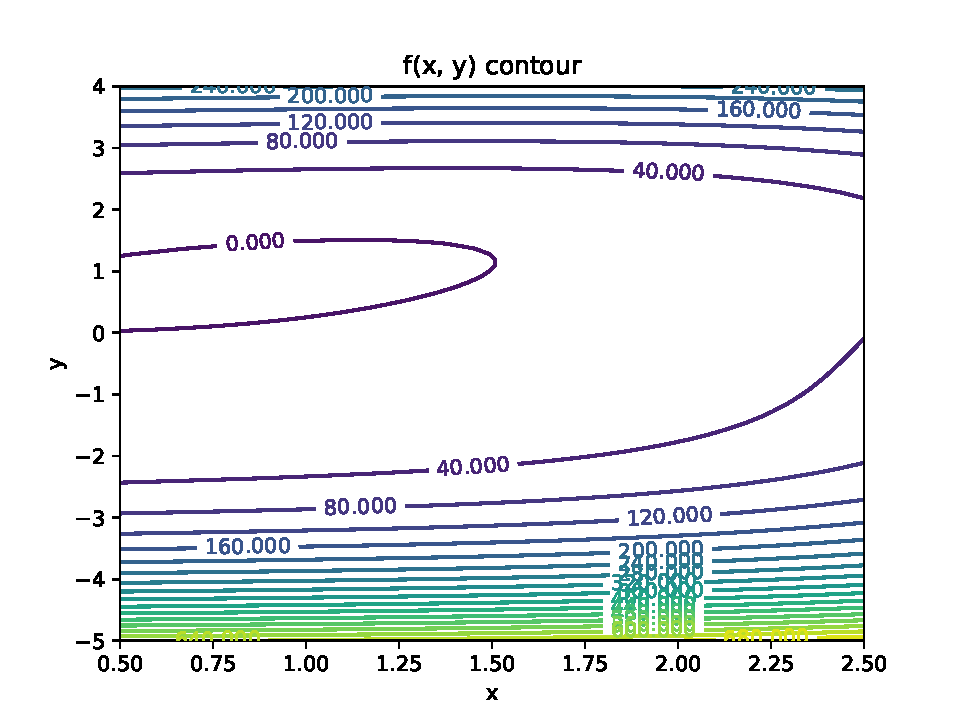
\includegraphics[page=1,width=.7\columnwidth]{figs/contour_21.pdf}
\caption{Contour Graph of $f(x, y)=x^{4}-4 x y+y^{4}$}
\end{figure}
\begin{figure}[t]
    \label{fig:example12_solution}
    \centering
    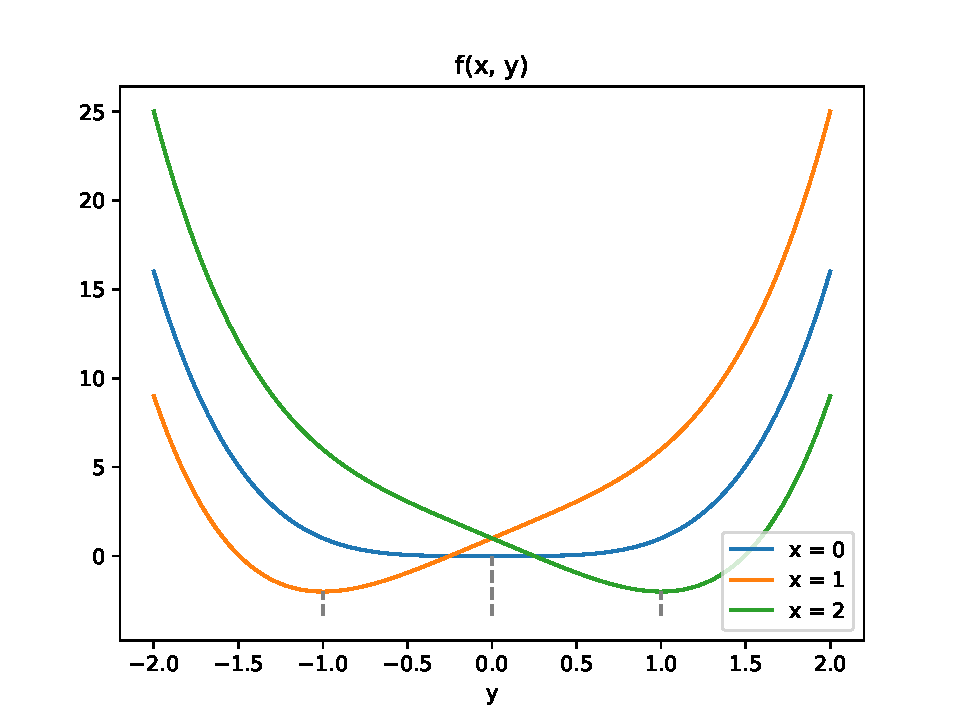
\includegraphics[page=1,width=.7\columnwidth]{figs/solution_21.pdf} 
  \caption{Function $f(x,y)$ at $x = 0$, $x=-1$ and $x=1$ }
 \end{figure}

\par From this example, we verify that through (NC1), we can find the global minimizer. However, not all continuous functions with critical points have any maximizer or minimizer. If the function goes to infinity along its axes or a line, it does not have any maximizer or minimizer although it has a critical point. The condition of the minimizer as the critical point is that the function $f$ should be a convex function with continuous first partial derivatives.
\par Let us move to the sufficient condition (SC1). The result obtained under this theorem is best possible for general functions. Specifically, for a convex function $f$ is defined on a convex set $\Omega \subset \mathbb{R}^n$, any local minimizer of f is also a global minimizer. Moreover, if a function $f$ is strictly convex, it has at most one global minimizer. 

\subsection{Optimality Conditions for Constrained Problems}
A general formulation for constrained optimization problems is as follows: 
\begin{equation}
\label{equ:2.2}
\begin{array}{l}\textrm { minimize } f(x) \\ \textrm { subject to }\left\{\begin{array}{ll}c_{i}(x)=0 & \textrm { for } i=1, \cdots, m_{e}, \\ c_{i}(x) \leq 0 & \textrm { for } i=m_{e}+1, \cdots, m\end{array}\right.\end{array}
\end{equation}
where $f$ and $c_i$ are smooth real-valued functions on $\mathbb{R}^n$, and $m_e$ and $m$ are nonnegative integers with $m_e < m$. We set 
$$
\mathscr{E}:=\left\{1, \cdots, m_{e}\right\} \quad \textrm { and } \quad \mathscr{I}:=\left\{m_{e}+1, \cdots, m\right\}
$$
as index sets of equality constraints and inequality constraints, respectively. 
\par Here, $f$ is so-called the objective function, and $c_i, i \in \mathscr{E} \textrm{ and } \mathscr{I}$ are equality constraints and inequality constraints respectively. 
\par To solve the optimization problem (\ref{equ:2.2}), we define the feasible set of it to be
$$
\mathscr{F}:=\left\{x \in \mathbb{R}^{n}: c_{i}(x)=0 \textrm { for } i \in \mathscr{E} \textrm { and } c_{i}(x) \leq 0 \textrm { for } i \in \mathscr{I}\right\}
$$
\par Any point $x \in \mathscr{F}$ is called a feasible point of (\ref{equ:2.2}) and we call (\ref{equ:2.2}) infeasible if $\mathscr{F} = 0$. Also, in this feasible set, a feasible point $x^* \in \mathscr{F}$ is called a local minimizer of (\ref{equ:2.2}) if it is the minimum solution in a neighborhood (strict local minimizer if it is the only one minimum solution). The definition of the global minimizer and strict global minimizer is similar, whose neighborhood is the whole feasible set. 
\par Let us move to the constraints in this problem. For equality constraints, they are strictly equivalent. However, for inequality constraints, there are some exceptions. Let $x^*$ be a local minimizer of (\ref{equ:2.2}). If there is an index $i \in \mathscr{I}$ such that $c_i(x^*) < 0$, then, $x^*$ is still the local minimizer of the problem obtained by deleting $i$-th constraint. In this situation, we say that the $i$-th constraint is inactive at $x^*$ since it does not have any effect on the solution. A general definition of active and inactive inequality constraints is as follows:
\begin{defn}
    At a feasible point $x \in \mathscr{F}$, the index $i \in \mathscr{I}$ is said to be \emph{active} if $\mathscr(x) = 0$ and \emph{inactive} if $c_i(x) < 0$.  
\end{defn}
\par In the next chapter, we will give different processes for different cases of active or inactive inequality constraints in the deep declarative nodes. In this chapter, we only focus on the necessary and sufficient conditions for a feasible point $x$ to be a local minimizer of (\ref{equ:2.2}). These conditions will be derived by considering the change of $f$ on the feasible set along with certain directions. We give the lemma for the condition of local minimizer $x^* \in \mathscr{F}$ as follows, which can be proved through Taylor’s formula in Appendix~\ref{appendix:lemma210}.
\begin{lemma}
    \label{lemma:210}
    If $x^* \in \mathscr{F}$ is a local minimizer of (\ref{equ:2.2}), then
    $$
    d^{T} \nabla f\left(x^{*}\right) \geq 0 \quad \textrm { for all } d \in T_{x^{*}} \mathscr{F}
    $$
    where $T_{x^{*}} \mathscr{F}$ is the set of all vectors tangent to $\mathscr{F}$. 
\end{lemma}
\par However, we may not be able to extract useful results from this lemma, since $T_{x^{*}} \mathscr{F}$ depends only on the geometry of $\mathscr{F}$ but not on the constraints functions $c_i$. Not all local minimum falls on the boundary of the constraint function, which is a part of $T_{x^{*}} \mathscr{F}$. Therefore, it is necessary to introduce linearized feasible directions to give a characterization of $T_{x^{*}} \mathscr{F}$ in terms of $c_i$. 
\begin{defn}
    \label{defn:lfd}
    Given $x \in \mathscr{F}$, we define
    $$
    \operatorname{LFD}(x):=\left\{d \in \mathbb{R}^{n}: d^{T} \nabla c_{i}(x)=0 \text { for } i \in \mathscr{E} ; d^{T} \nabla c_{i}(x) \leq 0 \textrm { for } i \in \mathscr{I} \cap \mathscr{A}(x)\right\}
    $$
    and call it the set of linearized feasible directions of $\mathscr{F}$ at $x$. 
\end{defn}
\par Heuristically, for $i \in \mathscr{E}$ we should travel along directions $d$ with $d^{T} \nabla c_{i}(x)=0$ in order to stay on the curve $c_i(x)=0$; for $i \in \mathscr{I}$ we should travel along directions with $d^{T} \nabla c_{i}(x) \leq 0$ in order to stay in the region $c_i(x) \leq 0$. 
Let us see an example of the linearized feasible directions and the tangent. Supposed we are considering a set $\mathscr{F}$ with variables $(x,y) \in \mathbb{R}^2$ and three inequality constraints functions: 
$$
\begin{aligned}
    c_1(x,y) &= x-1 \leq 0 \\
    c_2(x,y) &= -y \leq 0\\
    c_3(x,y) &= y^2 - x \leq 0
\end{aligned}
$$
\begin{figure}[t]
    \label{fig:example22_set}
    \centering
    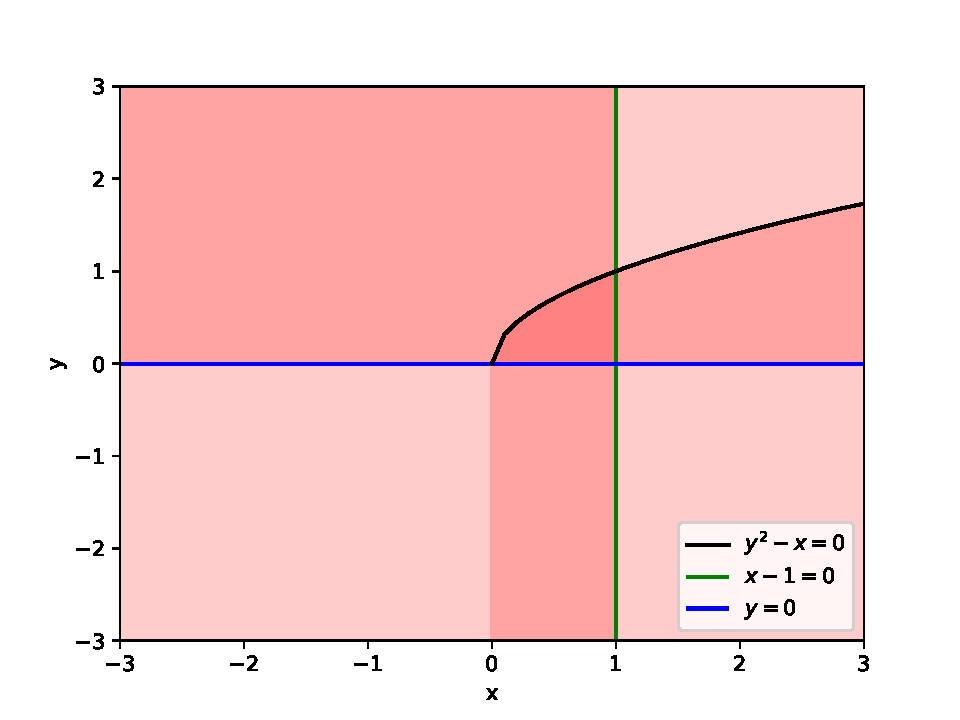
\includegraphics[page=1,width=.7\textwidth]{figs/solution_22.pdf} 
  \caption{Feasible set of constraints $c_1$, $c_2$ and $c_3$}
 \end{figure}

\par We can illustrate the feasible set of constriants $c_1$, $c_2$ and $c_3$ in Fig~\ref{fig:example22_set}. The active set of $0=(0,0)$ is $\{2, 3\}$, since $c_1(0) = -1 < 0$, which is inactive. And we can get the derivative of $c_2$ and $c_3$ at 0: 
$$
\nabla c_{2}(0)=(0,-1)^{T} \quad \textrm { and } \quad \nabla c_{3}(0)=(-1,0)^{T}
$$
\par Then we have the linearized feasible directions on $x=0$: 
$$
\begin{aligned} \operatorname{LFD}(0) &=\left\{d \in \mathbb{R}^{2}: d^{T} \nabla c_{2}(0) \leq 0 \text { and } d^{T} \nabla c_{3}(0) \leq 0\right\} \\ &=\left\{d \in \mathbb{R}^{2}: d \geq 0\right\} \end{aligned}
$$
which equals to the set of all vectors tangent to the feasible set $T_{0} \mathscr{F}$. 
\par Unlike the unconstrained optimization problem, the first order necessary condition of the existence of the optimizer is different since we should consider its linearized feasible directions and constraints feasibility. This is so-called the Karush-Kuhn-Tucker theorem: 
\begin{thm}[Karush-Kuhn-Tucker Theorem]
    \label{thm:kkt}
    Let $x^* \in \mathscr{F}$ be a local minimizer of problem (\ref{equ:2.2}). If
    $$
    T_{x^*} \mathscr{F} = \operatorname{LFD}(x^*),
    $$
    then there exists $\lambda^{*}=\left(\lambda_{1}^{*}, \cdots, \lambda_{m}^{*}\right)^{T} \in \mathbb{R}^{m}$ such that 
    $$
    \nabla f\left(x^{*}\right)+\sum_{i \in \mathscr{E} \cup \mathscr{I}} \lambda_{i}^{*} \nabla c_{i}\left(x^{*}\right)=0, \quad(\textrm {Lagrangian stationary})
    $$
    $$
    \left.\begin{array}{ll}c_{i}\left(x^{*}\right)=0 & \text { for all } i \in \mathscr{E}, \\ c_{i}\left(x^{*}\right) \leq 0 & \text { for all } i \in \mathscr{I},\end{array}\right\} \quad(\textrm {primal feasibility})
    $$
    $$
    \lambda_{i}^{*} \geq 0 \quad \textrm {for all} i \in \mathscr{I}, \quad (\textrm {dual feasibility})
    $$
    $$
    \lambda_i^*c_i(x^*) = 0 \quad \textrm {for all} i \in \mathscr{E} \cup \mathscr{I}. \quad (\textrm {complementary slackness})
    $$
    This set of equations are Karush-Kuhn-Tucker (KKT) conditions and a point $x^*$ is called a KKT point if there exists $\lambda^*$ such that $(x^*, \lambda ^*)$ satisfies the KKT conditions.
\end{thm}
\par For constrained optimization problem, the classic solution is using Lagrange multipliers \citep{BD:14}. This introduces the function 
$$
\mathscr{L}(x, \lambda):=f(x)+\sum_{i \in \mathscr{E} \cup \mathscr{I}} \lambda_{i} c_{i}(x)
$$
which is called the Lagrange function. $x$ is the primal variables and $\lambda_i, i=1, \dots, m$ are the Lagrange multipliers or the dual variables. According to the Lagrange multipliers method, we can solve this problem through the gradient of the Lagrange function: 
$$
\nabla_{x} \mathscr{L}(x, \lambda)=\nabla f(x)+\sum_{i \in \mathscr{E} \cup \mathscr{I}} \lambda_{i} \nabla c_{i}(x)
$$
\par Therefore, the first equation in KKT conditions can be written as
$$
\nabla_{x} \mathscr{L}\left(x^{*}, \lambda^{*}\right)=0
$$

\section{Solution of Unconstrained and Constrained Optimization Problems}
\label{sec:consopt}
According to the sufficient conditions for unconstrained optimization problems, we can easily compute the optimality through the first and second derivative of the objective function. For equality and inequality constrained problems, the introduction of Lagrangian $\mathcal{L}$ is useful for their closed-form solution. ~\cite{SG:16} collected both argmin and argmax bi-level optimization results with and without constraints, which also provide insightful examples of these cases. ~\cite{AB:17} also present a solution for exact, constrained optimization within a neural network. In this thesis, we only focus on argmin problems, but the argmax problems have similar results. 
\par In this section, we are going to provide some background for the solution of both unconstrained and constrained optimization problems, which is based on the gradient of the regular point. 
\subsection{Unconstrained Optimization}
For unconstrained optimization problems, the solution is easy to obtain since we only need to focus on the optimality of the objective function. We consider an objective function $f: \mathbb{R}^{n} \times \mathbb{R}^m \rightarrow \mathbb{R}$:
$$
y(x) \in \operatorname{argmin}f(x, y)
$$ 
\par The derivative of $y(x)$ with respect to $x$ is
\begin{equation}
\label{equ:2.3}
\frac{dy(x)}{dx} = -[\frac{\partial^{2} f}{\partial y(x)^{2}}]^{-1}\frac{\partial^{2} f}{\partial x \partial y(x)}
\end{equation}
which can be proved through differentiating and chain rule.~[\ref{appendix:equ2.3}]
\par A very classic example of the unconstrained minimization problem based on a closed convex nonempty set is the L2 norm $\|\cdot\|_2$. Let $\Omega \in \mathbb{R}^n$ be a closed convex nonempty set. For any $x \in \mathbb{R}^{n}$, the minimization problem is defined as follows:
$$
\min _{y \in \Omega}\|y-x\|_2^{2}
$$
\par This problem has a unique minimizer, which can be denoted by $P_\Omega(x)$, the Euclidean projection of $x$ onto $\Omega$. 
\begin{proof}
    Let $m:=\inf _{y \in \Omega}\|y-x\|_2^{2}$. Since $\Omega \neq \emptyset$, we have $0 \leq m < \infty$. Let $\{y_k\} \subset \Omega$ be a minimizing sequence such that $\left\|y_{k}-x\right\|_2^{2} \rightarrow m$ as $k \rightarrow \infty$. Thus $\left\|y_{k}-x\right\|_2^{2} \leq m+1$ for large $k$ which implies that $\left\|y_{k}\right\|_2 \leq\|x\|_2+\sqrt{m+1}$ for large $k$. Therefore $\{y_k\}$ is a bounded sequence. Consequently $\{y_k\}$ has a convegent subsequence  $\{y_{k_{l}}\}$ with limit $y^*$. Since $\Omega$ is closed, we have $y^* \in \Omega$, Thus
    $$
    m=\lim _{l \rightarrow \infty}\left\|y_{k_{l}}-x\right\|_2^{2}=\left\|y^{*}-x\right\|_2^{2}
    $$
    which means that $m$ is achieved at $y^*$, i.e. the given minimization problem has a solution. 
    \par Next we show that the given minimization problem has a unique solution by contradiction. If the solution is not unique, let $y_0$ and $y_1$ be two distinct solutions. Then for $0 < t < 1$ we set $y_{t}=t y_{1}+(1-t) y_{1}$. Since $\Omega$ is convex, we have $y_t \in \Omega$. Thus
    $$
    \begin{aligned}
        \left\|y_{0}-x\right\|_2^{2}=&\left\|y_{1}-x\right\|_2^{2} \leq\left\|y_{t}-x\right\|_2^{2}=\left\|t\left(y_{1}-x\right)+(1-t)\left(y_{0}-x\right)\right\|_2^{2} \\
        =& t^{2}\left\|y_{1}-x\right\|_2^{2}+(1-t)^{2}\left\|y_{0}-x\right\|_2^{2}+2 t(1-t)\left\langle y_{1}-x, y_{0}-x\right\rangle \\
        =& t\left\|y_{1}-x\right\|_2^{2}+(1-t)\left\|y_{0}-x\right\|_2^{2}-\left(t-t^{2}\right)\left\|y_{1}-x\right\|_2^{2} \\ 
        &-\left(1-t-(1-t)^{2}\right)\left\|y_{0}-x\right\|_2^{2}+2 t(1-t)\left\langle y_{1}-x, y_{0}-x\right\rangle \\
        =& t\left\|y_{1}-x\right\|_2^{2}+(1-t)\left\|y_{0}-x\right\|_2^{2} \\ 
        &-t(1-t)\left(\left\|y_{1}-x\right\|_2^{2}+\left\|y_{0}-x\right\|_2^{2}-2\left\langle y_{1}-x, y_{0}-x\right\rangle\right) \\
        =&\left\|y_{0}-x\right\|_2^{2}-t(1-t)\left\|y_{1}-y_{0}\right\|_2^{2} 
    \end{aligned}
    $$
    where $\langle\cdot, \cdot\rangle$ denotes the inner product on $\mathbb{R}^n$. Therefore $t(1-t)\left\|y_{1}-y_{0}\right\|_2^{2} \leq 0$ for $0 < t < 1$ and thus $\left\|y_{1}-y_{0}\right\|_2^{2} \leq 0$. So $y_1 = y_0$ 
    which is a contradiction. 
    \par Overall, the minimization problem defined above has a unique minimizer. 
\end{proof}
\par There are many different methods to solve the unconstrained optimization problem since generally, we treat this kind of problem as basic one. There are two most classical methods, Newton method~\citep{NT:36} and the Method of Steepest Descent~\citep{DP:09}. The former one, Newton method starts from an initial guess $x_0$ and defines a sequence $\{x_k\}$
iteratively according to some rule. It uses the tangent line of the objective function $f$ at $x_k$ to replace $f$ and uses the root of $L(x) = 0$, where $L(x)$ is the updated $f(x)$ as the next iterate $x_{k+1}$. Finally, the iteration is terminted as long as the difference between $x_k$ and $x_{k+1}$ less than a preassigned small number. The later one, steepest descent is a basic gradient method, which decreases the value of the objective function in a direction of most rapid change. The change rate of a function $f$ at $x$ in the direction $u$, a unit vector in $\mathbb{R}$ is determined by the directional derivative. Therefore, at $x$ the value of $f$ decrease fastest in the direction $u=-\nabla f(x)/\|\nabla f(x)\|$, which leads to the gradient method: we update the $x$ through the direction with the step length. 


\subsection{Equality Constrained Optimization}
Constrained problems are usually more complicated since the solution is restricted on a boundary or in a feasible region. For equality constraints, the basic case is the linear equality constraints $A \boldsymbol{y} = \boldsymbol{b}$. Again, we consider an objective function $f: \mathbb{R}^{m} \times \mathbb{R}^{n} \rightarrow \mathbb{R}$. Let $A \in \mathbb{R}^{p \times m}$ and $b \in \mathbb{R}^{p}$. $A$ is a set of $p$ linear equations as constraints $A \boldsymbol{y} = \boldsymbol{b}$. The problem is defined as follows:
$$
\begin{array}{rl}y(x) \in \arg \min _{y \in \mathbb{R}^{m}} & f(x, y) \\ \textrm { subject to } & A \boldsymbol{y}=\boldsymbol{b}\end{array}
$$
\par The derivative of $y(x)$ with respect to $x$ is
\begin{equation}
    \label{equ:2.4}
    \frac{dy(x)}{dx} = \left(H^{-1} A^{T}\left(A H^{-1} A^{T}\right)^{-1} A H^{-1}-H^{-1}\right) B
\end{equation}
where $H = \partial^{2} f(x, y) / \partial y(x)^2$ and $B = \partial^{2} f(x, y) / \partial x \partial y(x)$. 
\par The solution in~\ref{equ:2.4} can be proved through the Lagrange multipliers~\citep{BD:14} in ~\ref{appendix:equ2.4}. 
More generally, constraints can be non-linear. That means we cannot use $A$ as a weight matrix for constrained parameters anymore. Therefore, we define the equality constraints problem using a set of $m$ constraints functions $c(x, y)$: 
$$
\begin{array}{rl}y(x) \in \arg \min _{y \in \mathbb{R}^{m}} & f(x, y) \\ \textrm { subject to } & c_i(x, y) = 0, \quad i = 1, \dots, m \end{array}
$$
\par Solution for general multiple non-linear equality constraints is discussed in the chapter of deep declarative network nodes. Here, we are giving a simple example of non-linear equality constrained optimization problem. 
\par For any given nonzero vector $y \in \mathbb{R}^n$, we define the minimization problem as follows:
$$
\begin{array}{cc}\textrm { minimize } & -x^{T} y \\ \textrm { subject to } & \|x\|_{2}^{2}=1\end{array}
$$

\begin{figure}[t]
    \label{fig:example23_cons}
    \centering
    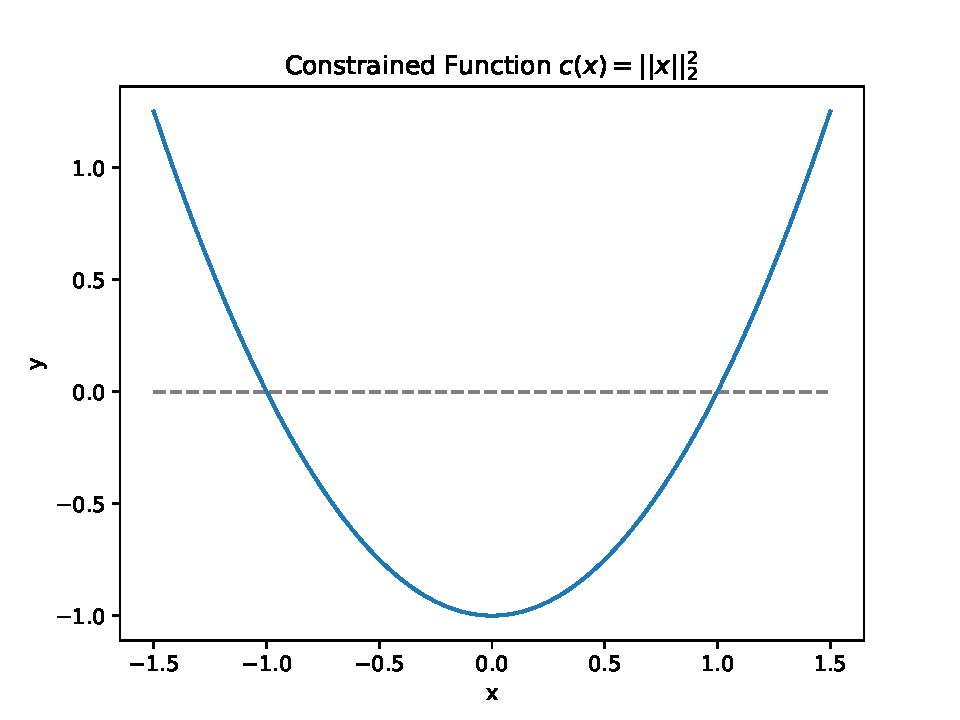
\includegraphics[page=1,width=.7\textwidth]{figs/constrained_22.pdf} 
  \caption{Constrained function $c(x) = \|x\|_{2}^{2} - 1$}
 \end{figure}

\par From the constraint defined above, we can write the constraint function as $c(x) = \|x\|_{2}^{2} - 1$ and illustrate it in Fig~\ref{fig:example23_cons}.  Differentiating $c(x)$ with respect to $x$, we get $\nabla c(x) = x \neq 0$. Therefore, it follows the definition of LFD~\ref{defn:lfd} and the theorem of KKT~\ref{thm:kkt}, which means that every local minimizer of this problem is a KKT point. Now we can write the Lagrangian function:
$$
\mathcal{L}(x, \lambda)=-x^{T} y+\lambda\left(\|x\|_{2}^{2}-1\right)
$$
and the KKT conditions are:
$$
\nabla_x \mathcal{L} = -y+2\lambda x = 0, \quad \|x\|_{2}^{2} = 1
$$
From $-y+2\lambda x = 0$ and $y \neq 0$ defined in the question, we must have $\lambda \neq 0$ and $x = y / 2\lambda$. Combined with $\|x\|_{2}^{2} = 1$, we get 
$$ 
4 \lambda^{2}=\|y\|_{2}^{2} \Leftrightarrow \lambda=\pm \frac{\|y\|_{2}}{2}
$$
\par Therefore, consequently, we have $x = \pm \frac{y}{\|y\|_{2}}$. For each $x$, we can compute its corresponding value of the objective function:
$$
x = \frac{y}{\|y\|_{2}}, -x^{T} y=-\|y\|_{2}
$$
$$
x = -\frac{y}{\|y\|_{2}}, -x^{T} y=\|y\|_{2}
$$ 
\par Obviously, the minimum is achieved $-\|y\|_{2}$ at $x = \frac{y}{\|y\|_{2}}$. 
\par Algorithms for solving constrained problems are various. For basic linear programming, which means that all functions involved are linear, we can transform it into standard form with matrix $A$, then solve the problem using Lagrangian function based on the KKT condition. 
\par Penalty method\citep{YO:05}, a function determining when a point $x$ is feasible or not, is used to replace the constrained problem with an unconstrained one. For a minimization problem $f(x)$, the penalty function $P(x)$ associated with a penalty parameter are introduced to combine with $f(x)$ and now we are going to solve a series of unconstrained problems. These problems have converged solutions of the original constrained problem. 

\subsection{Inequality Constrained Optimization}
Similar to equality constrained problems, inequality constrained problem usually defined the solution in a feasible set. In general, the standard form of inequality constrained problem is negative constraints:
$$
\begin{array}{rl}y(x) \in \arg \min _{y \in \mathbb{R}^{m}} & f(x, y) \\ \textrm { subject to } & c_i(x, y) \leq 0, \quad i = 1, \dots, m \end{array}
$$
\par Solutions for inequality constrained problems are various. According to the properties of inequality constraints, active and inactive constraints have different criteria. We aim to find the gradient of the optimal solution, $f\prime (x)$, based on the inequality constrained argmin function. 
 \cite{PE:88} proposed a globally convergent algorithm for solving the minimization of smooth objective function based on smooth inequality constraints. This algorithm is based on the Quasi-Newton~\citep{DJ:77} iteration for the solution of the first order condition of the optimality in KKT. An updated verision of this algorithm, a new QP-free method demonstrated by \cite{QH:00}, emphasizes the feasibility of all iterates. It reformulates the KKT optimality condition Fischer–Burmeister function~\citep{JH:99} for nonlinear complementarity problems. The classical solution is still based on the Lagrange multipliers. \cite{BD:14} proposed that for one-sided inequality constrained problems, it cannot be converted to equality constrained problem. Therefore, it introduced the method minimizing the augumented Lagrangian with respect to $x$ for various value of the Lagrange parameters, which is presented by \cite{PM:69} and \cite{HM:69}: 
 $$
 \begin{aligned} \bar{L}_{c}(x, z, \lambda, \mu)=& f(x)+\lambda^{\prime} h(x)+\frac{1}{2} c|h(x)|^{2} \\ &+\sum_{j=1}^{r}\left\{\mu_{j}\left[g_{j}(x)+z_{j}^{2}\right]+\frac{1}{2} c\left|g_{j}(x)+z_{j}^{2}\right|^{2}\right\} \end{aligned}
 $$
 \par The minimization of this augumented Lagrangian can be found through computing the first order derivative with respect to $z$ explicitly for each fixed $x$. 
\par More recently, \cite{SG:16} introduced a method approximating the gradient of the inequality constrained problem based on ideas from interior-point methods~\citep{BS:04}. It gives a demonstration of log-barrier function, which transforms the original constrained problem into a unconstrained minimization problem.
\begin{equation}
\label{equ:log-barrier}
\phi(x, y)=\sum_{i=1}^{m} \log \left(-c_{i}(x, y)\right)
\end{equation}
\begin{equation}
\label{equ:2.6}
\operatorname{minimize}_{y} \quad t f(x, y)-\sum_{i=1}^{m} \log \left(-c_{i}(x, y)\right)
\end{equation}
Equation~\ref{equ:log-barrier} is the log-barrier function, which takes the sum of the logrithm for all constraints. Then substracting it in the unconstrained minimization problem approximates the original inequality constrained problem. $t$ in Equation~\ref{equ:2.6} is a scaling factor for duality gap control if the solution set is convex. 
\par Similar to the solution for unconstrained and equality constrained problem, minimizing Equation~\ref{equ:2.6} is based on the gradient and hessian of the log-barrier function. Therefore, we can compute the approximation of the inequality constrained objective function. 

\section{Differentiable Neural Network}
\label{sec:differentiable}
If a problem is differentiable, that means the solution of this problem can be backpropagated. In neural networks, backpropagation~\citep{GI:16} is widely used to train the feedforward neural network, especially for supervised learning. Therefore, in deep neural networks, we can treat constrained optimization as an individual layer. Recently, there are several works on end-to-end differentiable convex optimization in the neural network, since this type of layer provides inductive bias for different problems, which is very practical. 
\par OptNet~\citep{AB:17} is a very classical differentiable layer neural network. Each layer in the end-to-end deep neural network is intergraded into optimization problems, which can capture and encode complex dependencies and constraints between hidden variables. It specifically considers the quadratic programs, which are general convex optimization problems. Similarly, SATNet~\citep{WP:19}, a differentiable maximum satisfiability solver, is also intergraded into end-to-end deep learning systems. Besides, it combines the solver with the traditional convolutional network. Both OptNet and SATNet are applied to solving the Sudoku puzzles, which is a very basic constrained logical problem. To make it more general and efficient, \cite{AA:19} demonstrate an approach based on disciplined convex programs, which is a subclass of the classical convex optimization problems. The affine map introduced in this paper represents the disciplined parametrized program. 
\par A fashion application in the differentiable network is the Perspective-n-Points (PnP) solver. \cite{CB:20} present BPnP based on PnP solver, performing geometric optimization in computer vision tasks. It backpropagates gradient through PnP accurately and effectively since there is a differentiable function in the optimizer block. Besides, for blind PnP problems in the 3D computer vision task, \cite{CD:20} propose an end-to-end network based on the differentiating optimization solutions, which is robust and outperforming.  
\par Apart from the above, the differentiable neural network has many practical and powerful applications. \cite{AB:19} introduce a differentiable variant cross-entropy method for non-convex optimization objective function. Again, due to the differentiable feature of the network, the output of the cross-entropy method is differentiable with respect to the parameters in the objective function, even it is non-convex. In 3D reconstruction tasks, some implicit shape and texture are difficult to represent. Hence, \cite{NM:20} introduce a differentiable rendering formulation, which makes the network learn them from input images directly since implicit differentiation can learn the depth gradients. Also, some research has been done to simplify the differentiable neural network since the computational cost and complexity of the differential operators can be very high in different tasks. The architecture proposed by \cite{CR:19} is cheap and efficient, which sets the Jacobian matrix into diagonal and hollow. It also changes the backward progress into automatic differentiation, which is more effective and lightweight. 


\section{Summary}
\label{sec:2summary}
In Chapter~\ref{cha:overviewpart1}, firstly, introduce the numerical optimization briefly with some necessary conditions and theorems. For the general convex optimization problem, the existence of the local or global optimizers can be determined by the feasible set. Next, the optimality of both unconstrained and constrained problems are discussed. For unconstrained problems, we only need to follow the necessary and sufficient conditions to find the global minimum of the solution. For constrained problems, it should also satisfy the KKT condition. Then we compare existing algorithms on the solution to these problems. Here, for constrained optimization problems, we have to consider the linearity of constraints. Specifically, the activity of inequality constraints can also be solved with different algorithms. Finally, since this thesis is based on the end-to-end differentiable network, some related works of the application are described since these works inspire the deep declarative network in the next chapter. In the next chapter, we are going to describe the deep declarative network in detail with examples. 





\chapter{Deep Declarative Network}
\label{cha:ddn}
In this chapter, we will cover the structure and nodes in the deep declarative network: from its learning process to the back-propagation.
\par Before delving into the details of the back-propagation in different constraints cases, we give an overview of the deep declarative network in Section~\ref{sec:overview-ddn}. In particular, the basic structure of the network and the details of declarative nodes are described according to \cite{SG:19}. The learning progress of the network is also given. We hope this will give readers a better sense of what is the deep declarative network and how it works. 
\par In Section~\ref{sec:bp}, we present the details of the back-propagation in different constrained problems. The gradient computation results are based on the implicit differentiation and different in constrained problems. We discuss this part based on the regular solution and compare it with the general solution in the previous chapter. 
\par Next we present the examples of constrained optimization problems with both linear and non-linear, equality and inequality constraints in Section~\ref{sec:example}. We also provide more implementation details of the deep declarative nodes. 
\par Finally, we summarize the deep declarative network and its solution in different constrained problems under the regular point. 


\section{An Overview of Deep Declarative Network}
\label{sec:overview-ddn}
\subsection{Declarative Node}
In deep declarative network, it defines the solution of a constrained optimization problem with parameter $x \in \mathbb{R}^n$ as the output of each node $y \in \mathbb{R}^m$. The general optimization problem can be defined as 
\begin{equation}
    \label{equ:ddn-basic}
    y \in \underset{u \in C}{\arg \min } f(x, u)
\end{equation}
where $f$ is the objective function $f: \mathbb{R}^n \times \mathbb{R}^m \rightarrow \mathbb{R}$, and $C \in \mathbb{R}^m$ is the set of constraints parameterized by $x$. 
\par Apart from the traditional forward processing mapping node, deep declarative node does not explicitly define the transforming function from the input to the output. It defines the input-output relationship implicitly by an objective and constraints optimization problem, where the solution of the problem is the output. 
\begin{figure}
    \label{fig:ddn}
    \centering
    \tikzset{every picture/.style={line width=0.75pt}} %set default line width to 0.75pt        

    \begin{tikzpicture}[x=0.75pt,y=0.75pt,yscale=-1,xscale=1]
    %uncomment if require: \path (0,300); %set diagram left start at 0, and has height of 300

    %Rounded Rect [id:dp5847695584847934] 
    \draw   (233,118.5) .. controls (233,113.81) and (236.81,110) .. (241.5,110) -- (421,110) .. controls (425.69,110) and (429.5,113.81) .. (429.5,118.5) -- (429.5,177.14) .. controls (429.5,181.84) and (425.69,185.64) .. (421,185.64) -- (241.5,185.64) .. controls (236.81,185.64) and (233,181.84) .. (233,177.14) -- cycle ;
    %Straight Lines [id:da8797940676718146] 
    \draw    (197.5,135.64) -- (230.5,135.64) ;
    \draw [shift={(232.5,135.64)}, rotate = 180] [color={rgb, 255:red, 0; green, 0; blue, 0 }  ][line width=0.75]    (10.93,-3.29) .. controls (6.95,-1.4) and (3.31,-0.3) .. (0,0) .. controls (3.31,0.3) and (6.95,1.4) .. (10.93,3.29)   ;
    %Straight Lines [id:da5288114309680509] 
    \draw    (232.5,165.64) -- (200.5,165.64) ;
    \draw [shift={(198.5,165.64)}, rotate = 360] [color={rgb, 255:red, 0; green, 0; blue, 0 }  ][line width=0.75]    (10.93,-3.29) .. controls (6.95,-1.4) and (3.31,-0.3) .. (0,0) .. controls (3.31,0.3) and (6.95,1.4) .. (10.93,3.29)   ;
    %Straight Lines [id:da8485926924080154] 
    \draw    (429.5,135.64) -- (462.5,135.64) ;
    \draw [shift={(464.5,135.64)}, rotate = 180] [color={rgb, 255:red, 0; green, 0; blue, 0 }  ][line width=0.75]    (10.93,-3.29) .. controls (6.95,-1.4) and (3.31,-0.3) .. (0,0) .. controls (3.31,0.3) and (6.95,1.4) .. (10.93,3.29)   ;
    %Straight Lines [id:da8644978866807145] 
    \draw    (463.5,165.64) -- (431.5,165.64) ;
    \draw [shift={(429.5,165.64)}, rotate = 360] [color={rgb, 255:red, 0; green, 0; blue, 0 }  ][line width=0.75]    (10.93,-3.29) .. controls (6.95,-1.4) and (3.31,-0.3) .. (0,0) .. controls (3.31,0.3) and (6.95,1.4) .. (10.93,3.29)   ;
    %Straight Lines [id:da03877231252818136] 
    \draw    (300,78.5) -- (300,107.64) ;
    \draw [shift={(300,109.64)}, rotate = 270] [color={rgb, 255:red, 0; green, 0; blue, 0 }  ][line width=0.75]    (10.93,-3.29) .. controls (6.95,-1.4) and (3.31,-0.3) .. (0,0) .. controls (3.31,0.3) and (6.95,1.4) .. (10.93,3.29)   ;
    %Straight Lines [id:da34598442566525556] 
    \draw    (350,109.64) -- (350,80.64) ;
    \draw [shift={(350,78.64)}, rotate = 450] [color={rgb, 255:red, 0; green, 0; blue, 0 }  ][line width=0.75]    (10.93,-3.29) .. controls (6.95,-1.4) and (3.31,-0.3) .. (0,0) .. controls (3.31,0.3) and (6.95,1.4) .. (10.93,3.29)   ;

    % Text Node
    \draw (260,140) node [anchor=north west][inner sep=0.75pt]   [align=left] {$\displaystyle y\ \in \underset{u\ \in \ C}{\arg\min} f( x,\ u;\ \theta ) \ $};
    % Text Node
    \draw (175,130) node [anchor=north west][inner sep=0.75pt]   [align=left] {$\displaystyle x$};
    % Text Node
    \draw (145,158) node [anchor=north west][inner sep=0.75pt]   [align=left] {$\displaystyle \operatorname{D} J( x)$};
    % Text Node
    \draw (475,130) node [anchor=north west][inner sep=0.75pt]   [align=left] {$\displaystyle y$};
    % Text Node
    \draw (472,158) node [anchor=north west][inner sep=0.75pt]   [align=left] {$\displaystyle \operatorname{D} J( y)$};
    % Text Node
    \draw (295,58) node [anchor=north west][inner sep=0.75pt]   [align=left] {$\displaystyle \theta $};
    % Text Node
    \draw (332,55) node [anchor=north west][inner sep=0.75pt]   [align=left] {$\displaystyle \operatorname{D} J( \theta )$};
    \end{tikzpicture}

    \caption{End-to-end learnable declarative node~\citep{SG:19}}
\end{figure}
\par Figure~\ref{fig:ddn} shows the forward and backward pass of the declarative node. In the forward evaluation pass, the output of the declarative $y$ is computed as the solution of some minimization problem $f(x, u; \theta)$. We use $\operatorname{D}$ to denote the total derivative with respect to the independent variables. Therefore, in the backward pass, the gradient of the global objective function with respect to the output $\operatorname{D}J(y)$ is back-propagated. Its value is computed through the chain rule based on the gradients with respect to the input $\operatorname{D}J(x)$ and parameters $\operatorname{D}J(\theta)$.
\par Since the definition of deep declarative nodes is very general, it can be embedded within another network for solving subproblems such as robust fitting. However, we may not be able to find the gradient when the feasible set is discrete, or the declarative node is low efficiency to evaluate. As non-regular solution cases, the nonexistent gradient problem will be discussed in the next part. In the next subsection, the learning details of the deep declarative network are described. 

\subsection{Learning}
Since in declarative nodes, there is no explicit forward function defined, we can directly compute the optimal solution $y$ through some algorithms. Under this assumption, when we performing the back-propagation, we can compute the gradient of the output from each node with respect to the corresponding input through the implicit differentiation directly. This can be treated as a bi-level optimization problem\citep{BJ:98} where the parameterized constraints as a lower-level problem blinds variables in the objective function, an upper-level problem. Combining the schematic illustration in Figure~\ref{fig:ddn}, the problem can be defined formally as
\begin{equation}
    \begin{array}{ll}\operatorname{minimize} & J(x, y) \\ \text { subject to } & y \in \arg \min _{u \in C} f(x, u)\end{array}
\end{equation}
\par We may have additional layers to make the objective function $J(x, y)$ depend on $y$, which is a function of $x$. In general, it is the sum of loss terms and regularization terms. We can solve this minimization problem through the gradient descent as follows:
\begin{equation}
    \operatorname{D}J(x,y) = \operatorname{D}_XJ(x,y) + \operatorname{D}_YJ(x,y)\operatorname{D}y(x)
\end{equation}
where $\operatorname{D}_XJ(x,y)$ is the partial derivatives of $J(x,y)$ with respect to $x$ and $\operatorname{D}_YJ(x,y)$ is the partial derivatives of $J(x,y)$ with respect to $y$. We used to use $\operatorname{D}_X$ and $\operatorname{D}_Y$ to denote the partial derivatives. We decompose the total derivatives of $J(x,y)$ as the sum of the partial derivatives with the chain rule. In application, we can consider it as the sum of gradients for losses on training examples. 
\par The lower-level objective function $f$ can be simpler. If it is the only term involving $y$ in the upper-level objective function $J$, that means $J(x,y) = g(x, f(x,y))$ and the lower-level problem is actually unconstrained with $u \in C=\mathbb{R}^m$. Under this condition, the calculation of the gradient can be expanded using chain rule through both $\operatorname{D}_XJ(x,y)$ and $\operatorname{D}_YJ(x,y)$:
\begin{equation}
    \begin{aligned} 
        \operatorname{D} J(x, y) &=\operatorname{D}_{X} g(x, f)+\operatorname{D}_{F} g(x, f)\left(\operatorname{D} f+\operatorname{D}_{Y} f \operatorname{D} y\right) \\ &=\operatorname{D}_{X} g(x, f)+\operatorname{D}_{F} g(x, f) \operatorname{D} f 
    \end{aligned}
\end{equation}
where $\operatorname{D}_Yf(x,y) = 0$ since $y$ is the minimum of $f(x,y)$ and $f(x,y)$ is an unconstrained problem, its partial derivative should be zero. 
\par In addition, for the solution $y$, we should verify its regularity. 
\begin{defn}[Regular Point]~\citep{SG:19}
    \label{defn:regular-point}
    A feasible point $u$ is said to be \emph{regular} if the equality constraints gradient $D_Uh_i$ and the active inequality constraints gradients $D_Ug_i$ are linearly independent, or there are no equality constraints and the inequality constraints are all inactive at $u$.
\end{defn}
Therefore, in unconstrained problems, we can consider the solution is regular by default. However in constrained problems, especially the inequality constrained problems, we should be aware of the feasible set is continuous or not. 

\section{Back-propagation Through Declarative Nodes}
\label{sec:bp}
Let us focus back on the more general case with $y$ involving in different terms. The backward pass is different in different sub-classes of declarative nodes. We consider three common cases based on Equation~\ref{equ:ddn-basic}. 

\subsection{Unconstrained}
Firstly, the most basic case is the unconstrained problem. Consider a function $f: \mathbb{R}^n \times \mathbb{R}^m \rightarrow \mathbb{R}$, we have
\begin{equation}
    y \in \underset{u \in C}{\arg \min } f(x, u)
\end{equation}
\par We make the assumption that the solution of this problem, $y(x)$ exists, and in the neighborhood of the point $(x, y(x))$, $f$ is second-order differentiable. Therefore, we can compute the derivative of $y$ with respect to $x$ is
$$
\operatorname{D}y(x) = -H^{-1}B
$$
where $H = \operatorname{D}_{YY}^2 f(x, y(x)) \in \mathbb{R}^{m \times m}$ is the second-order derivative of $f$ with respect to $y$, and it is a non-singular matrix. $B = \operatorname{D}_{XY}^2 f(x, y(x)) \in \mathbb{R}^{m \times n}$ is the second-order derivative of $f$ with respect to $y$ and $x$ (the derivative of $D_Yf(x,y)$ with respect to $x$). 
\par The proof of this solution is similar to the proof of Equation~\ref{equ:2.3}: setting the partial derivative of $f(x,y)$ with respect to the optimal $y$ as 0, then transposing and differentiating both sides according to the implicit function theorem: 
\begin{equation}
    \begin{aligned} 
        0_{m \times n} &=\operatorname{D}\left(\operatorname{D}_{Y} f(x, y)\right)^{T} \\ &=\operatorname{D}_{X Y}^{2} f(x, y)+\operatorname{D}_{Y Y}^{2} f(x, y) \operatorname{D} y(x) 
    \end{aligned}
\end{equation}
After rearrangement, we get
\begin{equation}
    \operatorname{D} y(x)=-\left(\operatorname{D}_{Y Y}^{2} f(x, y)\right)^{-1} \operatorname{D}_{X Y}^{2} f(x, y)
\end{equation}
\par Since this is the unconstrained case, for any stationary point of $f(x,y)$, the result is valid. In the following constrained cases, the optimal solution is actually the stationary point of the Lagrangian. 

\subsection{Equality Constrained}
Secondly, we consider the equality constrained problem, that means the feasible set is defined by $p$ nonlinear equality constraints. Consider functions $f: \mathbb{R}^n \times \mathbb{R}^m \rightarrow \mathbb{R}$ and $h: \mathbb{R}^n \times \mathbb{R}^m \rightarrow \mathbb{R}^p$, we have
\begin{equation}
    \begin{aligned} 
        y(x) \in & \arg \min _{u \in \mathbb{R}^{m}} f(x, u) \\ & \text { subject to } \quad h_{i}(x, u)=0, i=1, \ldots, p 
    \end{aligned}
\end{equation}
where $h = [h_1, \dots, h_p]^T$ are a set of constraints. 
\par Again, we make the assumption that the solution of this problem, $y(x)$ exists and both $f$ and all constraints in $h$ are second-order differentiable. Also, we should consider the Jacobian matrix of $h$ with respect to $y$ is full rank since we need the optimal point is regular. Then we can calculate the derivative of $y$ with respect to $x$ is
$$
\operatorname{D} y(x)=H^{-1} A^{T}\left(A H^{-1} A^{T}\right)^{-1}\left(A H^{-1} B-C\right)-H^{-1} B
$$
where
$$
\begin{aligned} 
    A &=\operatorname{D}_{Y} h(x, y) \in \mathbb{R}^{p \times m} \\ B &=\operatorname{D}_{X Y}^{2} f(x, y)-\sum_{i=1}^{p} \lambda_{i} \operatorname{D}_{X Y}^{2} h_{i}(x, y) \in \mathbb{R}^{m \times n} \\ C &=\operatorname{D}_{X} h(x, y) \in \mathbb{R}^{p \times n} \\ H &=\operatorname{D}_{Y Y}^{2} f(x, y)-\sum_{i=1}^{p} \lambda_{i} \operatorname{D}_{Y Y}^{2} h_{i}(x, y) \in \mathbb{R}^{m \times m} 
\end{aligned}
$$
and $\lambda \in \mathbb{R}^p$ can be solved through the system $\lambda ^T A = \operatorname{D}_Yf(x,y)$. 
\par Similar to the solution of linear equality constrained problem in Equation~\ref{equ:2.4}, we can form the Lagrangian by the method of Lagrange multipliers\citep{BD:14}:
\begin{equation}
    \mathcal{L}(x, y, \lambda)=f(x, y)-\sum_{i=1}^{p} \lambda_{i} h_{i}(x, y)
\end{equation}
\par We introduce the Lagrange multipliers $\lambda$ to set the stationary point of this Lagrangian is $(y, \lambda)$. Then we differentiate $\mathcal{L}$ with respect to $y$ and $\lambda$ separately, which are both resulting in 0 since $y$ is the optimality. We have two cases at the optimal point $y$. The first one is that the partial derivatives of $f$ with respect to $y$ equals to zero: $\operatorname{D}_Yf(x,y) = 0 \in \mathbb{R}^{1 \times m}$. That means we transfer this problem to an unconstrained problem since its solution satisfies the constraints directly. Under this case, $\lambda$ can be set as 0 directly. The second one is that the partial derivatives of $f$ with respect to $y$ is non-zero vector, and it is orthogonal to the constraint surface, which is controlled by the set of equality constraints $h(x, y) = 0$. In this case, from the derivative of $\mathcal{L}$ with respect to $y$ equaling to zero, we have
\begin{equation}
    \mathrm{D}_{Y} f(x, y)=\sum_{i=1}^{p} \lambda_{i} \mathrm{D}_{Y} h_{i}(x, y)=\lambda^{T} A
\end{equation}
where $A$ is the same as the defined above. 
\par To solve this equation for $\lambda$, if we want to compute explicitly, it has a unique analytic solution $\lambda = (AA^T)^{-1}A(\operatorname{D}_Yf)^T$. 

\par Next, we compute the second-order derivative of $\mathcal{L}$ with respect to $x$. It still equals to zero in both functions. Solving the equation through variable elimination~\citep{BS:04} we have
\begin{equation}
    \operatorname{D} \lambda(x)=\left(A H^{-1} A^{T}\right)^{-1}\left(A H^{-1} B-C\right)
\end{equation}

\begin{equation}
    \label{equ:solution-eq}
    \operatorname{D} y(x)=H^{-1} A^{T}\left(A H^{-1} A^{T}\right)^{-1}\left(A H^{-1} B-C\right)-H^{-1} B
\end{equation}
which is our result. 
\par The problem and solution defined in Section~\ref{sec:equ-opt} is the simplier case of this general one. Also, if we only have one constraint, the matrix $A$ and vector $\lambda$ can be simplifed as vector and scalar separately. Moreover, for linear only constraints, the repsentation of matrix $H$ and $B$ are also simper since $\lambda = 0$.  

\subsection{Inequatlity Constrained}
Lastly, inequality constrained problems are more complicated since we have to consider the solution for active and inactive constraints. Also, previous works metioned in Section~\ref{sec:ineq-opt} are approximation results or focusing on the convex problems. Here, the declarative nodes consider the the problem containing both equality and inequality constraints. Consider functions $f: \mathbb{R}^n \times \mathbb{R}^m \rightarrow \mathbb{R}$ and $h: \mathbb{R}^n \times \mathbb{R}^m \rightarrow \mathbb{R}^p$, and $g: \mathbb{R}^n \times \mathbb{R}^m \rightarrow \mathbb{R}^q$, we have
\begin{equation}
    \begin{aligned} 
        y(x) \in & \arg \min _{u \in \mathbb{R}^{m}} f(x, u) \\ & \text { subject to } \quad\begin{array}{l}h_{i}(x, u)=0, i=1, \ldots, p \\ g_{i}(x, u) \leq 0, i=1, \ldots, q\end{array}
    \end{aligned}
\end{equation}
where $h = [h_1, \dots, h_p]^T$ are still a set of equality constraints, and $g = [g_1, \dots, g_q]^T$ are a set of inequality constraints. 
\par In declarative nodes, it present a more general result based on activity of all inequality constraints at the optimal point $y(x)$. Also, assumptions of the existence of the optimal point $y(x)$ and second-order differentiation of $f$, $g$, $h$ remain true. We combine the equality constraints and inequality constraints together in $\tilde{h} = [h_1, \dots, h_p, g_1, \dots, g_q]$ and the derivative of $\tilde{h}$ with respect to $y$ is a full rank matrix to keep the regularity. We have
\begin{equation}
    \label{equ:solution-ineq}
    \operatorname{D} y(x)=H^{-1} A^{T}\left(A H^{-1} A^{T}\right)^{-1}\left(A H^{-1} B-C\right)-H^{-1} B
\end{equation}
where
$$
\begin{aligned} 
    A &=\operatorname{D}_{Y} \tilde{h}(x, y) \in \mathbb{R}^{(p+q) \times m} \\ B &=\operatorname{D}_{X Y}^{2} f(x, y)-\sum_{i=1}^{p} \lambda_{i} \operatorname{D}_{X Y}^{2} \tilde{h}_{i}(x, y) \in \mathbb{R}^{m \times n} \\ C &=\operatorname{D}_{X} \tilde{h}(x, y) \in \mathbb{R}^{(p+q) \times n} \\ H &=\operatorname{D}_{Y Y}^{2} f(x, y)-\sum_{i=1}^{p+q} \lambda_{i} \operatorname{D}_{Y Y}^{2} \tilde{h}_{i}(x, y) \in \mathbb{R}^{m \times m} 
\end{aligned}
$$
and $\lambda \in \mathbb{R}^{p+q}$ satisfies $\lambda ^T A = \operatorname{D}_Yf(x,y)$ with $\lambda_i \leq 0$ for $i = p+1, \dots, p+q$, which is almost the same as the solution of the equality constrained problem. 

\begin{figure}
    \label{fig:regular-point}
    \centering
    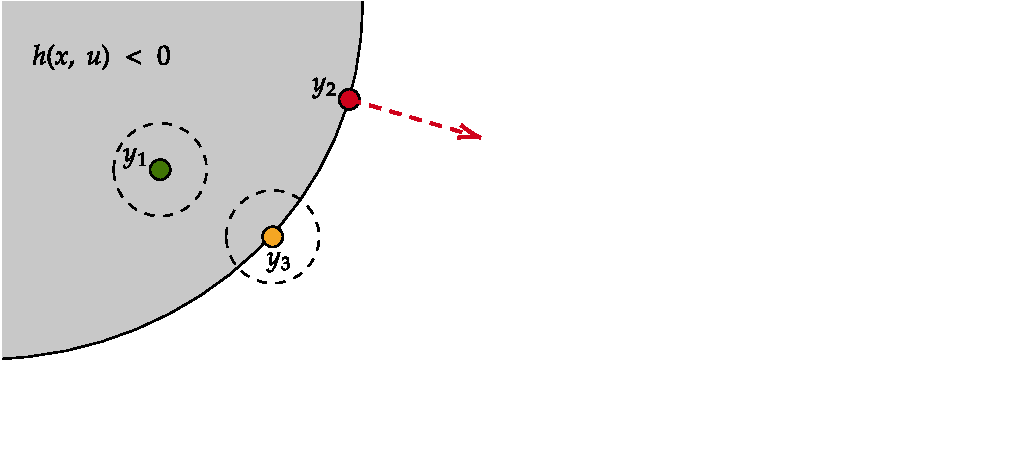
\includegraphics[]{figs/non-regular-scenario.pdf}
    \caption{Different scenarios for the solution to inequality constrained nodes}
\end{figure}

\par However, in inequality constraints, the gradient is discontinuous since the Lagrange multipliers $\lambda$ for active inequality constraints are zero. We separate the solution of inequality constrained declarative nodes into 3 scenarios, which is illustrated in Figure~\ref{fig:regular-point}. For any inequality constraints $g(x, u) \leq 0$, the constraint can be active or inactive at the optimal solution $y$. In the first scenario, the constraint is inactive at the solution $y$, which means $g(x,y) < 0$ and it is completely in the feasible set ($y_1$). Therefore we have $\operatorname{D}_Yf(x,y) = 0$ and we can consider it as an unconstrained problem. In the second scenario, the constraint is active at $y$, but it is orthogonal to the constraint surface ($y_2$). Then we have $\operatorname{D}_Yf(x,y) \neq 0$ and $\lambda \neq 0$. Then we can consider this inequality constraint as an equality one since the solution falls on the boundary of the feasible set, but the gradient of negative and pointing outside the set. The last scenario, the constraint is active and $\operatorname{D}_Yf(x,y) = 0$ when the solution is on the boundary and it is a local minimum ($y_3$). For the backward propagation, in this case, we can choose both solutions of unconstrained or equality constrained gradient. 

\section{Examples of Declarative Nodes}
\label{sec:example}
\subsection{Implementation Details}
We give the implementation of both equality and inequality constraints with linear and nonlinear cases in raw Python under the gradient calculation package Autograd\citep{MD:15}. In this subsection, we are going to show the implementation details of the basic deep declarative nodes.
\par \textbf{Constraints definition.}  
In the multiple equality constraints node and inequality constraints node, equality constraints and inequality constraints are defined in two functions separately. If there are more than one constraint, they are stored in a 1-d array. All constraints equal to zero or less than 0, which means all parameters in the equations are in the left-hand side and the right-hand side is always zero. There is a specific checking function defined to check this. In the linear equality constraints node, the set of linear constraints are defined as a single matrix $A$ and its corresponding vector $b$ in the initialization directly. 

\par \textbf{Gradient computation.}
To compute the gradient of the solution under the constraints, we need to calculate the Jacobian and Hessian matrix, which are the first-order and second-order derivative matrix of the constraints. For matrix $H$ in the general solution of the constrained problem, it is costly to compute the inverse of it. Therefore, we transfer the problem to solving a linear system $Hx_1 = A^T$ and $Hx_2 = B$ where $x_1 = H^{-1}A^T$ and $x_2 = H^{-1}B$ to solve them. Cholesky decomposition, an algorithm for solving the linear system efficiently, is applied to this problem. It decomposes a Hermitian positive-definite matrix into the product of a lower triangular matrix with real and positive diagonal entries with its conjugate transpose, which is the unique decomposition. In our problems, since matrix $H$ is a symmetric real positive-definite matrix, it can be decomposed through this algorithm effectively. The solution of the Lagrange multipliers $\lambda$ similar, which is the solution of a linear system $\lambda^T A = \operatorname{D}_Yf(x,y)$ through the least-square solution solver. 
\par \textbf{Optimality checking.} For constrained optimization problems, according to the optimality conditions defined in Section~\ref{sec:opt-con-constrained}, we should check if the first-order optimality condition is satisfied or not. We define a function in all cases for checking the optimality: the gradient of constraint is zero at optimal point ($\operatorname{D}_Yh(x,y) = 0$), or the gradient of objective function equals to the product of the Lagrange multipliers and the gradient of constraints ($\operatorname{D}_Yf(x, y) = \lambda \operatorname{D}_Yh(x, y)$). 

\par \textbf{Exception handling.}
Since our assumptions are based on the regular solution, and not all problems have a regular optimal point, we define the exception cases for this problem. When we solve the linear system for the Lagrange multipliers $\lambda$, if the solution does not falls as a regular point, we may get a null value in $\lambda$ due to the non-existence of the gradient on a non-regular solution. We are going to discuss the solution for this specific case in the next part. For here, we just throw the exception once there is a null value in the Lagrange multipliers $\lambda$. 

\subsection{Equality Constrained}
Firstly, we consider a single linear equality constrained problem, minimizing the KL-divergence between the input $x$ and output $y$ subject to the output forming a valid probablility vector, which can be formally defined as 
\begin{equation}
    \begin{array}{rll}
        y =& \text{argmin}_u & - \sum_{i=1}^{n} x_i \log u_i \\
        & \text{subject to} & \sum_{i=1}^{n} u_i = 1
    \end{array}
\end{equation}
where the positivity constraint on $y$ is automatically satisfied by the domain of the log function.
\begin{figure}[t]
    \label{fig:equ-lin-eg}
    \centering
    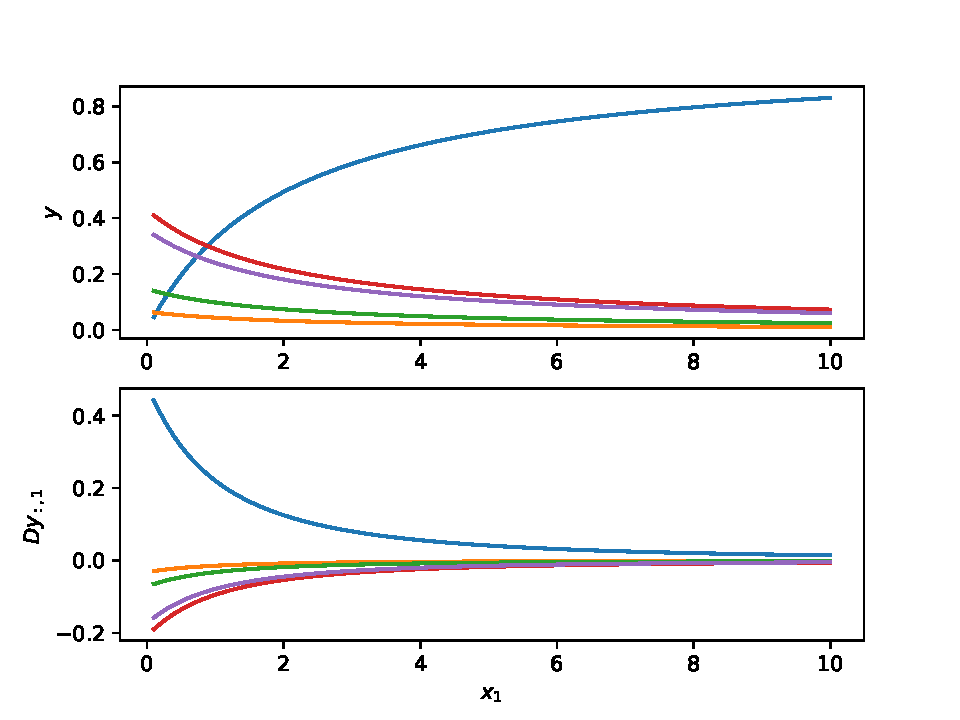
\includegraphics[page=1,width=.8\textwidth]{figs/linear_equality_example.pdf} 
    \caption{Plots of the function $y$ (top) and the gradient (bottom) sweeping the first component of the input $x_1$ while holding the other elements of $x$ constant}
\end{figure}
\par A nice feature of this problem is that we can solve it in closed-form as
$$
y = \frac{1}{\sum_{i=1}^{n} x_i} x.
$$

\par Now we are going to solve this problem via an iterative method with derivative of deep declarative node. Set $n=5$ and $m=5$, which means the input $x \in \mathbb{R}^5$ and the output $y \in \mathbb{R}^5$. We begin from a random feasible solution, which is the normalization of the value $y$, then preform the gradient update. Figure~\ref{fig:equ-lin-eg} shows the function and gradient sweeping the first component of the input $x_1$ from 0.1 to 10.0 while holding the other elements of $x$ constant. 
\par Now we consider a multiple non-linear equality constrained problem which is defined formally as
\begin{equation}
    \begin{array}{rll}
        y =& \text{argmin}_u & \sum_{i=1}^{n} x_i u_i^{2} \\
        & \text{subject to} & \sum_{i=1}^{n-1} u_i^2 = 1 \\
        & & \sum_{i=1}^{n} u_i = 0 \\
    \end{array}
\end{equation}
\begin{figure}[t]
    \label{fig:equ-nonlin-eg}
    \centering
    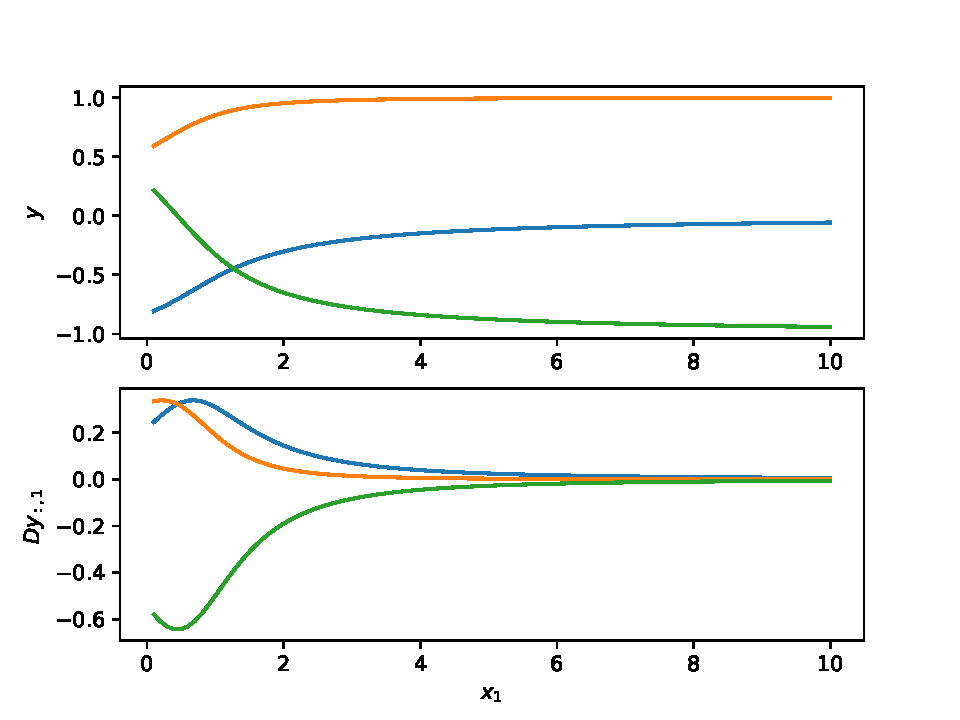
\includegraphics[page=1,width=.8\textwidth]{figs/multiple_equality_example.pdf} 
    \caption{Plots of the function $y$ (top) and the gradient (bottom) sweeping the first component of the input $x_1$ while holding the other elements of $x$ constant}
\end{figure}
\par Same as the previous example, we instantiate the multiple equality constriants nodes in deep declarative nodes with $n=3$ and $m=3$. We begin from a feasible solution, $\cos^2 x + \sin^2 x - \sin x - \cos x = 0$, performing the gradient descent until the convergence. Figure~\ref{fig:equ-nonlin-eg} shows the function $y$ and its gradient changes. 
\subsection{Inequatlity Constrained}
For inequality constrained problems, we consider a similar problem based on the multiple equality constrained problem above. The only difference is that we restrict the first parameter $u_1$ is less than $u_2$. Therefore, the problem is defined as
\begin{equation}
    \begin{array}{rll}
        y =& \text{argmin}_u & \sum_{i=1}^{n} x_i u_i^{2} \\
        & \text{subject to} & \sum_{i=1}^{n-1} u_i^2 = 1 \\
        & & \sum_{i=1}^{n} u_i = 0 \\
        & & u_1 - u_2 < 0
    \end{array}
\end{equation}
\begin{figure}[t]
    \label{fig:ineq-eg}
    \centering
    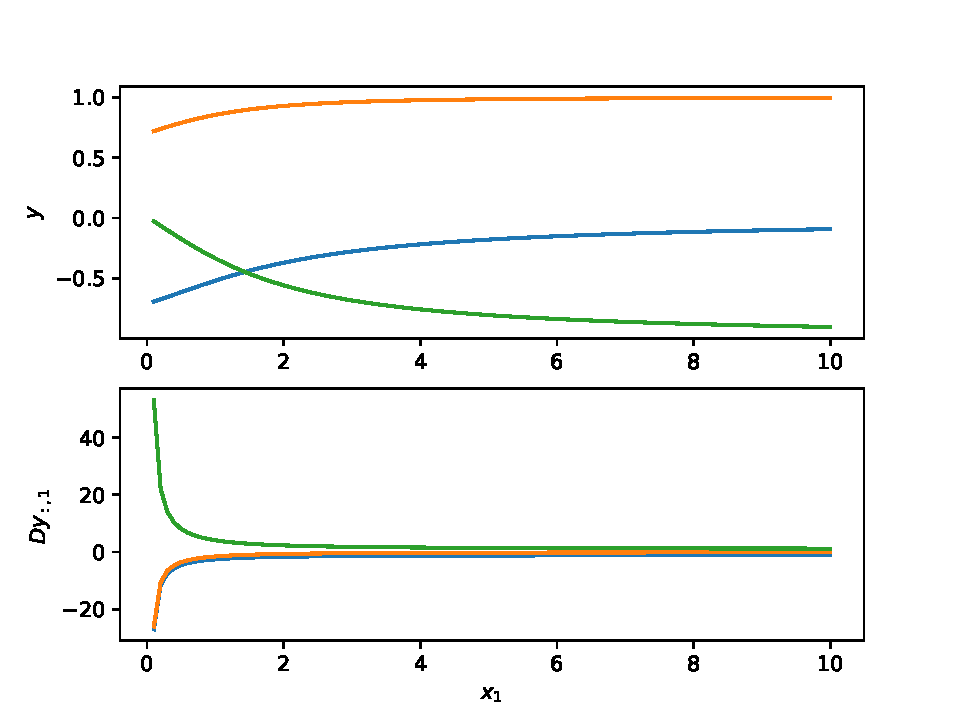
\includegraphics[page=1,width=.8\textwidth]{figs/multiple_inequality_example.pdf} 
    \caption{Plots of the function $y$ (top) and the gradient (bottom) sweeping the first component of the input $x_1$ while holding the other elements of $x$ constant}
\end{figure}
\par The deep declarative node is the instantiation of inequality constraints nodes with $n=3$ and $m=3$. Same as the feasible solution as the beginning, we set $x=\pi / 6$, which satisfies the inequality constraints since $\sin (\pi/6) < \cos (\pi/6)$. Figure~\ref{fig:ineq-eg} shows the function $y$ and its gradient changes. The gradient flattened to some extreme value at the beginning of the iteration then converge to almost zero. 

\section{Future Work of the Deep Declarative Network}
There are various possible challenging extensions of the deep declarative network in both theory and application. As a differentiable network, it combines the exact functionality solution with the iterative gradient method. In this section, we give several future foreseeable extensions of the declarative network comparing with other state-of-the-art differentiable models in both theory optimization and applications in computer vision tasks. 
\par We give the solution to the deep declarative nodes of constrained problems under the assumption that the solution of the problem $y(x)$ exists, and it should be a regular point whose gradient can be computed. Also, both objective function and constraints are required to be first and second-order differentiable, which also means that they are continuous instead of discrete. Therefore, in some computer vision tasks such as binary constrained classification problem may not be able to solve using this approach. Some relevant extension methods are discussed in PART II. Also, the robustness of the declarative nodes can be improved by introducing attention to specific constraints. 
\par In solving the real computer vision tasks, comparing to other differentiable models, the deep declarative network can be applied to the visual Sudoku problem. Also, many constrained optimization problems in the graph can be solved through this method. Future work in applications can focus on providing a more specific algorithm for different tasks. 

\section{Summary}
In Chapter~\ref{cha:ddn}, we describe the deep declarative network from its structure to its implementation with examples of different constrained problems. As a differentiable neural network, the deep declarative network defines its nodes to process input implicitly through the optimization problem, which can find the optimal solution directly without the verification of the local or global minimum. Its learning progress is also based on the derivative of the solution and the gradient of its constraints. We also introduce the back-propagation through deep declarative nodes in three subclasses: unconstrained, constrained, and inequality constrained problems. All representations of the gradient in declarative nodes have assumptions of the existence of the optimal point, its regularity, and its first and second-order derivative. In the next chapter, we are going to give an overview of the non-regular solution with related previous works. 
\chapter{The Future of Declarative Nodes}
\label{cha:futurepart1}
Same as the last chapter, introduce the motivation and the high-level picture to
readers, and introduce the sections in this chapter.

\section{Improvements of the Optimization}

\section{Applications in Computer Vision Tasks}


\part{Deep Declarative Network: Non-regular Solution}
\chapter{An Overview of Regular and Non-regular Solution}
\label{cha:overviewpart2}
In PART I, we described the solution for both unconstrained and constrained problems in deep declarative nodes: its theoretical background of numerical optimization, the general solution for unconstrained and constrained optimization problems, and the details of the back-propagation in deep declarative noes. However, the solutions given before are based on the assumption of the existence of the solution and the second-order differentiable objective functions and constraints. In PART II, we will extend the solution for different non-regular solutions which can approximate the gradient of constrained problems. 
\par In this chapter, we will give an overview of the non-regular point for deep declarative nodes with some related previous works. According to the definition of regular point in Definition~\ref{defn:regular-point}, we focus on the solution which is not regular, which means we cannot use the solutions we proposed in the previous chapter to solve them. 
\par We first discuss possible non-regular solutions problems in the deep declarative nodes in Section~\ref{sec:problems-in-non-regular}, with corresponding specific examples. Next, we briefly discuss several previous related works in solving non-regular points problems in Section~\ref{sec:relatedworknonreg}. Since we set this chapter as the background information of our solutions in the next chapter, we also provide some comparison between these existed approaches. 
\par We finally give a summary of the non-regular solution cases and our literature review findings. 


\section{Problems in Regular Deep Declarative Nodes}
\label{sec:problems-in-non-regular}

\subsection{Assumptions and Problems}
In Section~\ref{sec:bp}, we provided general solutions for unconstrained and constrained optimization problems in deep declarative nodes. For both problems, we assume that the solution of the problem, $y(x)$ exists in the neighborhood of the point $(x, y(x))$. Also, the objective function is supposed to be second-order differentiable. In particular, for constrained optimization problems, all constraints are also assumed to be second-order differentiable. These assumptions are made to guarantee that the optimal point is regular and strictly minimum. 
\par However, not all problems have differentiable constraints and the jacobian or hessian matrix of constraints is full-ranked. Also, the first-order derivatives of the equality constraints and active inequality constraints may not linear independent. The dimension of the output may also various from the number of active constraints. According to the solution of equality constraints and inequality constraints in Equation~\ref{equ:solution-eq} and Equation~\ref{equ:solution-ineq} with their corresponding representations of matrix $H$, we have to compute the inverse of the matrix $H$ to get the solution. If $H$ is singular or very sparse, we are not able to get the exact solution since we cannot apply the Cholesky decomposition to this matrix. 
\par There are many possible problems of non-regular solutions in the deep declarative nodes. We summarize them as three majority cases: Overdetermined system, rank deficiency problems, and non-convex cases. 

\subsection{Overdetermined System}
If the constraints we get are more than unknowns we are going to solve, this system of equations is considered overdetermined. In declarative nodes, we require at least one degree of freedom for the back-propagation, since we have to update the gradient with the direction in a feasible solution set. Therefore, when the number of active constraints exceeds the dimensionality of the output, the system is overdetermined. 
\begin{figure}[t]
    \label{fig:overdetermined-solution}
    \centering
    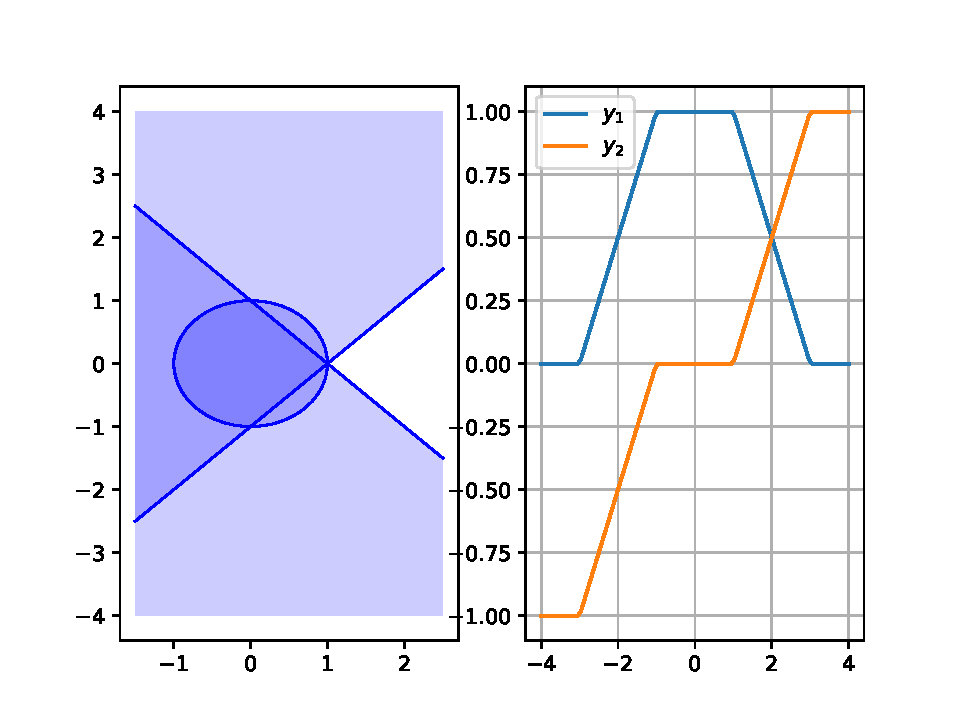
\includegraphics[page=1, width=.8\textwidth]{figs/overdetermined.pdf}
    \caption{The feasible solution set and the results of the overdetermined system}
\end{figure}
\par We give the first example constrains the solution to a circle with two segments removed in Figure~\ref{fig:overdetermined-solution}. Also, we formulate this as the intersection of a (solid) circle constraint with two half-spaces. The problem is defined officially as 
\begin{equation}
    \begin{array}{llll}
        y \in & \text{argmin}_u & \frac{1}{2} \|u - x\|^2 \\
        & \text{subject to} & u_1^2 + u_2^2 - 1 \leq 0 & (h_1) \\
        & & u_1 - u_2 - 1 \leq 0 & (h_2) \\
        & & u_1 + u_2 - 1 \leq 0 & (h_3)
    \end{array}
\end{equation}
From Figure~\ref{fig:overdetermined-solution}, there is only one intersection point among three constraints, where all three constraints are active. We calculate the graident of it using the implicit differentiation of the KKT optimality conditions as discussed in Equation~\ref{equ:solution-ineq} and their corresponding formulas. Figure~\ref{fig:overdetermined-gradient} shows the value of $y$ and the corresponding gradient. Using the solution for inequality constraints problems, we can get
$$
\begin{array}{llll}
    A &= \text{D}_{Y} h(y) &= \begin{bmatrix}
         2 y_1 & 2 y_2 \\ 1 & -1 \\ 1 & 1
         \end{bmatrix} & \text{for active $h_i$} \\
    B &= \text{D}^2_{XY} f(x, y) - \sum_{i=1}^{3} \lambda_i \text{D}^2_{XY} h_i(y) &= -I \\
    C &= \text{D}_{Y} h(y) &= 0 \\
    H &= \text{D}^2_{YY} f(x, y) - \sum_{i=1}^{3} \lambda_i \text{D}^2_{YY} h_i(y) &= (1 - 2 \lambda_1) I 
\end{array}
$$
\begin{figure}[t]
    \label{fig:overdetermined-gradient}
    \centering
    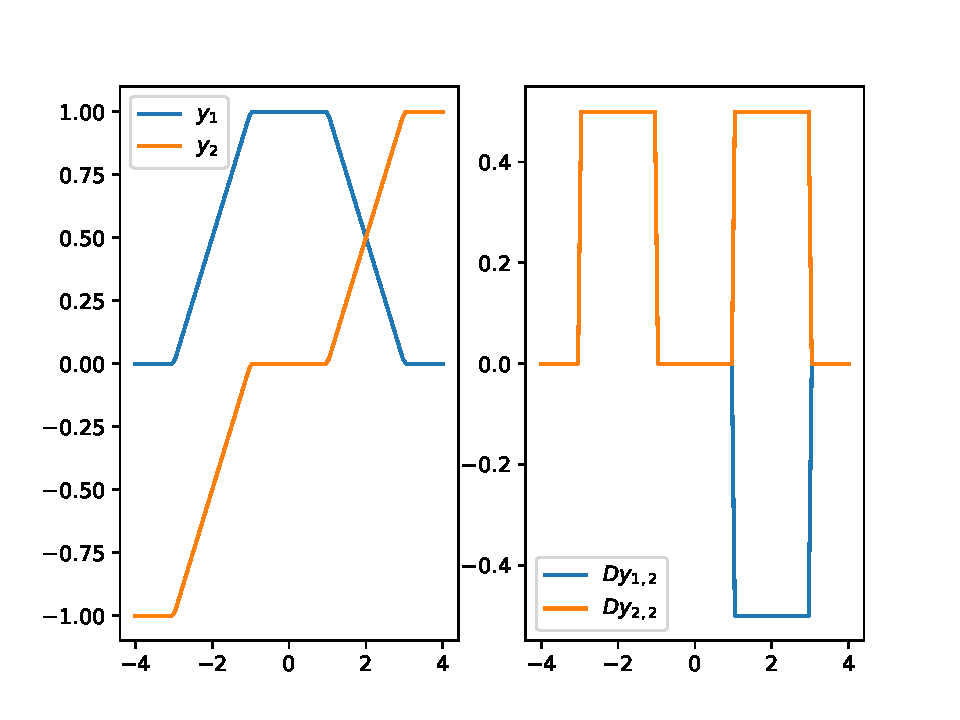
\includegraphics[page=1, width=.8\textwidth]{figs/overdetermined-gradient.pdf}
    \caption{The results and corresponding gradient solution of the overdetermined system}
\end{figure}
where inactive constraints, and corresponding Lagrange multipliers, are first removed. Thus, the matrix $A$ may have between zero and three rows, which is not regular. This equation can be solved to give different results: 
$$
\text{D} y(x) = \begin{cases}
        I & \text{if all constraints are inactive} \\
        0 & \text{if all constraints are active (since $C = 0$)} \\
        I - A^T (AA^T)^{-1} A & \text{if $h_1$ is inactive} \\
        \frac{1}{1 - 2 \lambda_1} \left(I - A^T (AA^T)^{-1} A\right) & \text{otherwise.}
    \end{cases}
$$
where the gradient is zero if all constraints are active. In this scenario, we can not perform back-propagation in our deep declarative network. 

\subsection{Rank Deficiency Problems}
Contrary to the overdetermined system, rank deficiency means that there are insufficient equations to determine the solution, which is the so-called underdetermined system. More generally, we do not have enough information to estimate the desired model in this case. 
\par In declarative nodes, if the first-order derivatives of the equality constraints and active inequality constraints are linearly dependent, the solution points are not regular since the KKT conditions may still be satisfied but there are degrees of freedom in the Lagrange multipliers. The direct result is that matrix $H$ is sparse and singular. 
\begin{figure}[t]
    \label{fig:rank-deficiency}
    \centering
    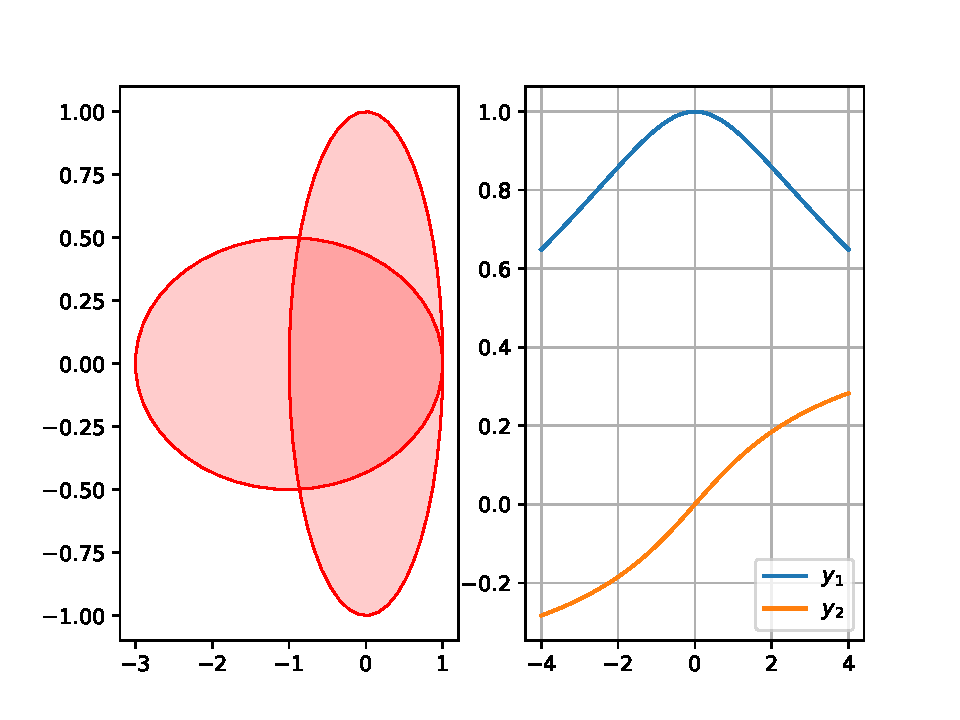
\includegraphics[page=1, width=.8\textwidth]{figs/rankdeficient.pdf}
    \caption{The feasible solution set and the results of the rank-deficiency problem}
\end{figure}
\par We give the example that the constraint set is defined as the intersection between a circle and an ellipse in Figure~\ref{fig:rank-deficiency}. The problem is defined officially as
\begin{equation}
    \begin{array}{llll}
        y \in & \text{argmin}_u & \frac{1}{2} \|u - x\|^2 \\
        & \text{subject to} & u_1^2 + u_2^2 - 1 \leq 0 & (h_1) \\
        & & \frac{1}{4}(u_1 + 1)^2 + 4 u_2^2 - 1 \leq 0 & (h_2)
    \end{array}
\end{equation}
where the solution $y \in \mathbb{R}^2$ is a function of $x$ and at $x_2 = 0$, both constraints are active. This results in $A$ being rank deficient. 
\par Similar to the previous overdetermined system, we can compute the gradient $\operatorname{D}y(x)$ of this rank deficient problem with each matrix as follows
$$
\begin{array}{lll}
    A &= \begin{bmatrix}
         2y_1 & 2 y_2 \\ \frac{1}{2} (y_1 + 1) & 8 y_2
         \end{bmatrix} & \text{for active $h_i$} \\
    B &= -I \\
    C &= 0 \\
    H &= \begin{bmatrix}
         1 - 2 \lambda_1 - \frac{1}{2} \lambda_2 & 0 \\
         0 & 1 - 2 \lambda_1 - 8 \lambda_2
         \end{bmatrix}
\end{array}
$$
where $A$ is rank deficient at $y = (1, 0)$. 

\begin{figure}[t]
    \label{fig:rank-deficiency-gradient}
    \centering
    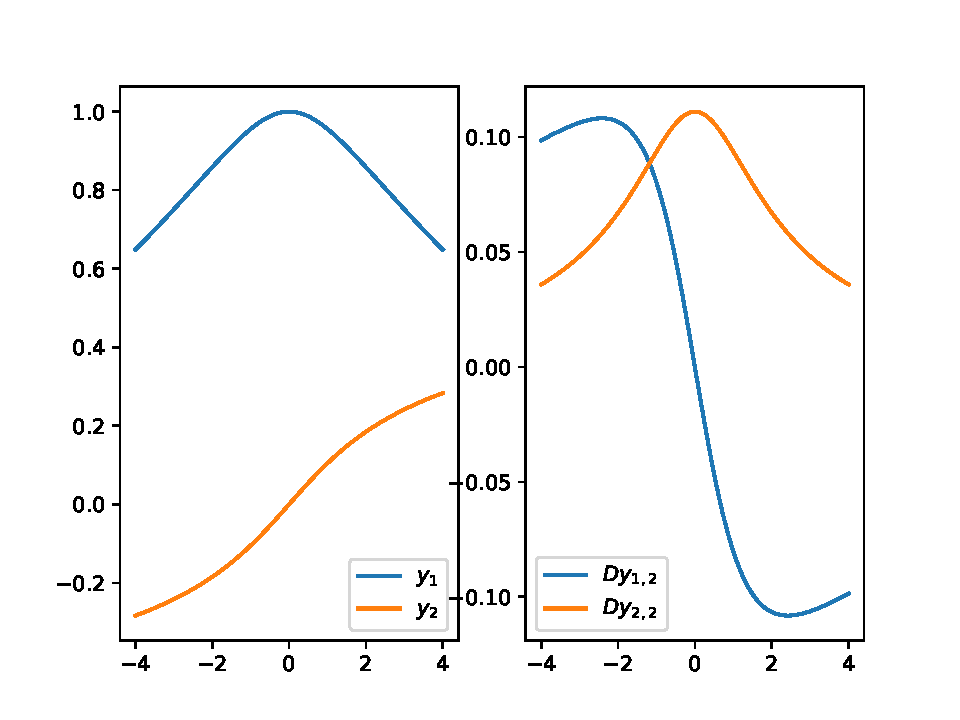
\includegraphics[page=1, width=.8\textwidth]{figs/gradient-rank-deficient.pdf}
    \caption{The results and corresponding gradient solution of the rank-deficiency problem}
\end{figure}
\par Since in $A$, some columns are linear dependent, here we need to remove one of the rows of $A$ before solving for $\operatorname{D}y(x)$. One strategy is to keep those constraints where the rate of change of the objective is steepest relative to the curvature induced by the constraint surface. That is, remove from $A$ rows that are linearly dependent on other rows and with the smaller $\text{D}_{Y}f (\text{D}_{YY}^2 h_i)^{-1} \text{D}_{Y}f^T$. Figure~\ref{fig:rank-deficiency-gradient} shows the solution of $y$ with their corresponding gradient. 

\subsection{Non-convex Cases}
The last scenario is the non-convex cases, which is also a rank deficient problem. In general, solving a non-convex problem is NP-hard since it potentially has many local minima or solutions are in very flat regions, which is hard to update the gradient. 
\par Similarly, we give the example that the constraint set is defined as the area in the circle that is not within the ellipse,
\begin{equation}
    \label{equ:non-convex}
    \begin{array}{llll}
        y \in & \text{argmin}_u & \frac{1}{2} \|u - x\|^2 \\
        & \text{subject to} & u_1^2 + u_2^2 - 1 \leq 0 & (h_1) \\
        & & \frac{1}{4}(u_1 + 1)^2 + 4 u_2^2 - 1 \geq 0 & (h_2)
    \end{array}
\end{equation}
\begin{figure}[t]
    \label{fig:non-convex}
    \centering
    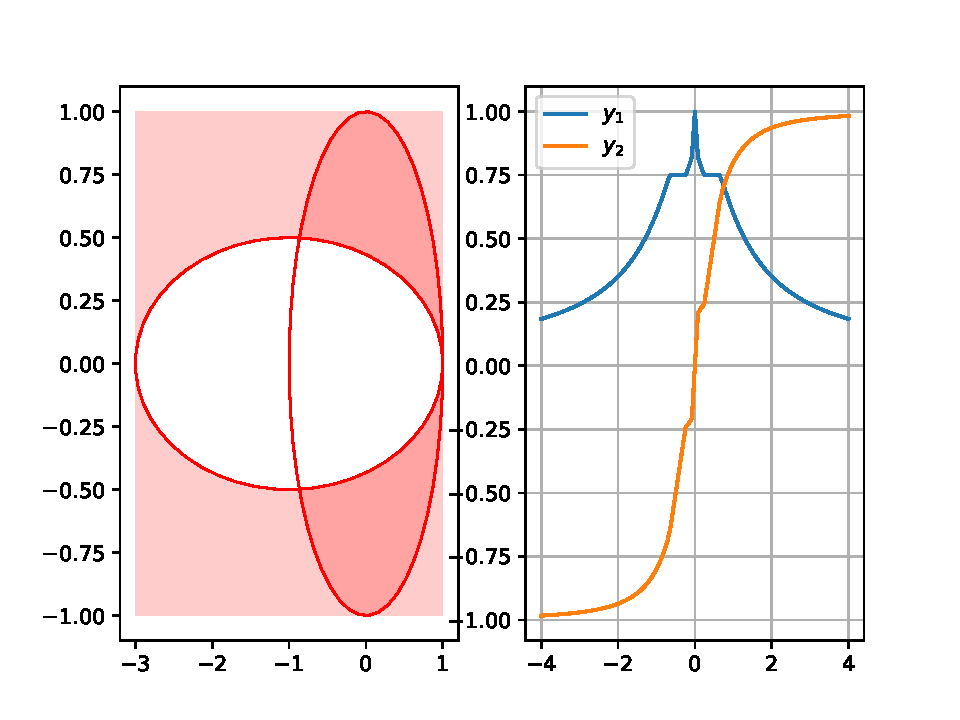
\includegraphics[page=1, width=.8\textwidth]{figs/nonconvex.pdf}
    \caption{The feasible solution set and the results of the non-convex case}
\end{figure}
\par Figure~\ref{fig:non-convex} shows the feasible solution set, which is non-convex of this problem and the results $y$ with fixed $x_1 =0.75$ and $x_2$ sweeping from -4 to 4. When $x = (0.75, 0)$, the result $y = (1, 0)$ and both constraints $h_1$ and $h_2$ in Equation~\ref{equ:non-convex} are active. Thus at this point, the matrix $A$ is deficient.
\begin{figure}[t]
    \label{fig:non-convex-gradient}
    \centering
    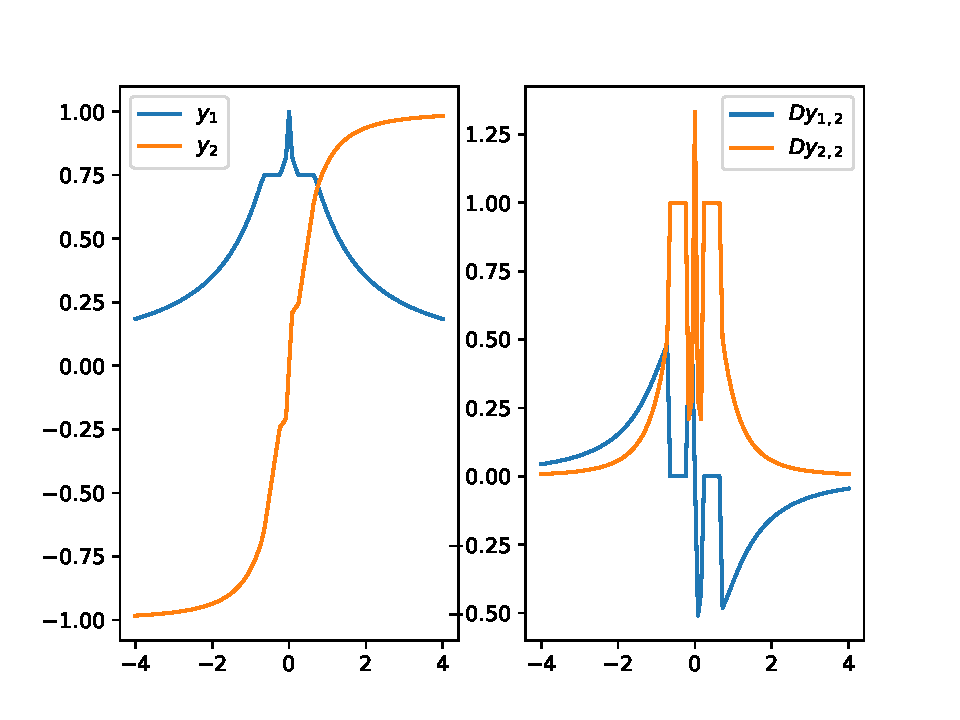
\includegraphics[page=1, width=.8\textwidth]{figs/gradient-non-convex.pdf}
    \caption{The results and corresponding gradient solution of the non-convex case}
\end{figure}
\par Now we use the same method to calculate the gradient $\operatorname{D}y(x)$, we have
$$
\begin{array}{lll}
    A &= \begin{bmatrix}
         2y_1 & 2 y_2 \\ -\frac{1}{2} (y_1 + 1) & -8 y_2
         \end{bmatrix} & \text{for active $h_i$} \\
    B &= -I \\
    C &= 0 \\
    H &= \begin{bmatrix}
         1 - 2 \lambda_1 + \frac{1}{2} \lambda_2 & 0 \\
         0 & 1 - 2 \lambda_1 + 8 \lambda_2
         \end{bmatrix}
\end{array}
$$
where $A$ is rank deficient at $y = (1, 0)$. Figure~\ref{fig:non-convex-gradient} shows the solution of $y$ with their corresponding gradient. 
\par We give an example for each non-regular solution scenario, which is not able to compute the gradient directly. In the next section, we discuss several previous related works in solving these problems. 

\section{Related Work in Non-regular Solution}
\label{sec:relatedworknonreg}
Most previous works in the differentiable network only focus on the regular and convex solution. However, to some extent, dealing with non-regular solutions is solving non-regular linear systems. Therefore, we present several related works in discussing the solution of the overdetermined system, rank deficient problems, and non-convex cases in linear equations. 
\par \textbf{Overdetermined system.} The approximation of the solution for the overdetermined system is various. The most classical approach is the ordinary least squares, which minimize the $L_2$ residual between $Ax$ and $b$~\citep{AH:13}. However, if we want to have more numerical accurate solutions, QR factorization can give better results~\citep{TL:97}. Besides, \cite{BI:74} proposed the solution in the $L_1$ norm for calculating those data contains wild points, which are unstable with $L_2$ norm. They also introduced an algorithm to solve the linear Chebyshev data fitting problem, which is also overdetermined~\citep{BI:75}. Apart from them, \cite{WG:79} demonstrated a minimax solution for the overdetermined system of nonlinear equations based on the minimax norm. All these methods are similar since they are implemented to minimize the error between the exact solution and the approximation. 
\par \textbf{Rank deficiency problems.} As an underdetermined system, many previous methods are provided through a similar approximation as the overdetermined system for the sparse matrix $A$. \cite{DD:05} demonstrated a method for finding the unique sparse solution by $L_1$ minimization and neighborliness of convex polytopes, which transferring the problem to a convex optimization problem. They also proved that the minimal $L_1$-norm solution is also the sparsest solution ~\citep{DD:06}. 



\section{Summary}

\chapter{Results}
\label{cha:result}




\section{Direct Cost}\
\label{sec:direct_cost}

Here is the example to show how to include a figure. Figure~\ref{fig:cost}
includes two subfigures (Figure~\ref{fig:zerocost}, and Figure~\ref{fig:zerobus});

\begin{figure*}
  \label{fig:cost}
  \subfigure[Fraction of cycles spent on zeroing\label{fig:zerocost}]{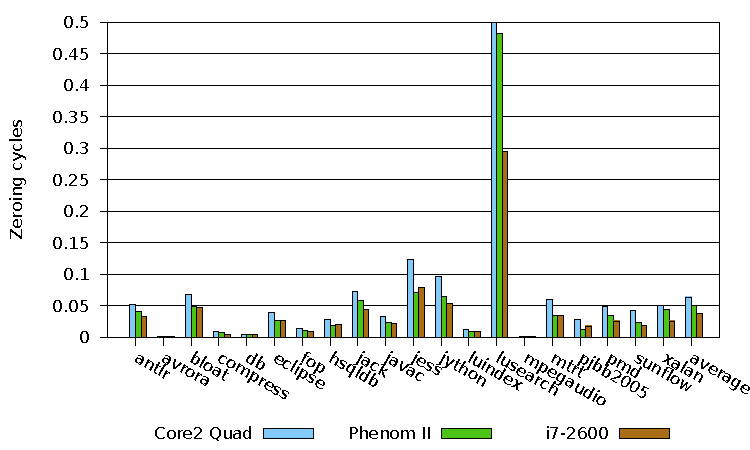
\includegraphics[width=\columnwidth]{figs/zerocost_intel.pdf}}
  \subfigure[BytesZeroed / BytesBurstTransactionsTransferred\label{fig:zerobus}]{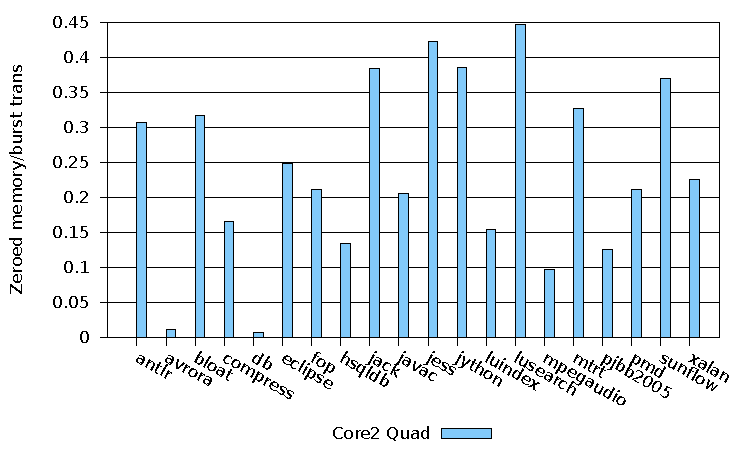
\includegraphics[width=1.0\columnwidth]{figs/zerobus_core.pdf}}
  \caption{The cost of zero initialization}
\end{figure*}


\section{Summary}

\chapter{Conclusion}
\label{cha:conc}
In this thesis, we gave readers a thorough overview of constrained optimization in the deep declarative network: the multiple constraints nodes (PART I) and solutions for non-regular points (PART II). 
\par In Chapter~\ref{cha:overviewpart1}, we walked through the theory of numerical optimization, which is the theoretical background of the deep declarative network. A system explanation of the optimality conditions of constrained optimization problems under the assumption of convexity is given: the objective function is differentiable at the optimal point and twice differentiable on the definition set. Solutions to unconstrained and constrained optimization problems are discussed, which are obtained based on the optimality conditions with Lagrange multipliers. We also introduced the related works in the differentiable network, which is different from the traditional deep neural network using the properties of back-propagation with differentiable optimization problems to construct the nodes.
\par In Chapter~\ref{cha:ddn}, we covered all contents of the deep declarative network. More specifically, the properties and functions of deep declarative nodes. We introduced how the deep declarative network works and its learning progress based on the end-to-end learnable declarative nodes. We later presented the back-propagation and corresponding gradient solution of regular points through declarative nodes in different scenarios: unconstrained, equality constrained and inequality constrained. We also showed various examples of our implementation of deep declarative nodes in different scenarios. We hope our works in this new type of differentiable network will eventually lead to a new generation of deep neural networks.
\par In PART II, the key questions we wanted to answer are: Is the solution of the deep declarative nodes always regular? If the solution is non-regular, how do we find the gradient then perform the back-propagation? 
\par In Chapter~\ref{cha:overviewpart2}, we addressed the problems in regular deep declarative nodes, which is based on the assumption of convexity in the optimality conditions. We separated the problems into three scenarios: the overdetermined system, rank deficiency problems and non-convex cases. We also provided the corresponding example for each scenario, which is not able to obtain the gradient directly. Lastly, we discussed multiple previous works in solving non-regular solution problems. 
\par In Chapter~\ref{cha:result}, we showed that we can deal with the different non-regular solutions with both approximation and theoretical based optimality methods. For overdetermined systems and rank deficiency problems, we introduced approaches based on the least-squares method and iterative gradient descent. Both of these methods try to approximate the closest solution with minimum residual errors. For non-convex cases, we proposed a different algorithm for solving the constrained optimization problems based on the optimality conditions regardless of the convexity. This technique can solve the problem exactly with the weighted Chebyshev norm and non-linear Lagrangian. We believe these methods are useful for handling all range of solutions in the deep declarative network. 
\par All together, we are really excited about the progress that has been made in this field for the past years and have been glad to be able to contribute to this field. At the same time, we also hope to encourage e more researchers to work on the applications, or apply the deep declarative network to new domains or tasks. We believe that it will lead us towards building better constrained problem solvers and hope to see these ideas implemented and developed in industry applications.

%%%%%%%%%%%%%%%%%%%%%%%%%%%%%%%%%%%%%%%%%%%%%%%%%%%%%%%%%%%%%%%%%%%%%%
% Here begins the end matter

%%\chapter{Appendix}
\renewcommand{\thesection}{\Alph{section}}
\label{appendix}
\section{An Overview of Numerical Optimization}
\subsection{Theory of Optimization}

\subsubsection{Proof of Theorem~\ref{thm:23}}
\label{appendix:trm23}
\begin{proof}
Let 
$$
m:=\inf \{f(x): x \in \Omega\}
$$
By the definition of $m$ we may pick a sequence $\left\{x_{k}\right\} \subset \Omega$ with $f\left(x_{k}\right) \rightarrow m$ as $k \rightarrow \infty$. Because $\Omega$ is compact, we can extract a convergent subsequence $\left\{x_{k_j}\right\}$ from $\left\{x_{k}\right\}$. Let $x^{*} \in \Omega$ denote the limit point of $\left\{x_{k_j}\right\}$. Since $f$ is continuous, $f\left(x^{*}\right)=\lim _{j \rightarrow \infty} f\left(x_{k_{j}}\right)=m$. Thus $m$ is finite and $x^{*}$ is a global minimizer of $f$ on $\Omega$. \\
When $\Omega = \mathbb{R}^n$, we need to impose conditions on f at infinity to guarantee the existence of a global minimizer.
\end{proof}

\subsubsection{Proof of Theorem~\ref{thm:24}}
\label{appendix:trm24}
\begin{proof}
Let $m:=\inf \left\{f(x): x \in \mathbb{R}^{n}\right\}$, and take a sequence $\left\{x_{k}\right\}$ such that 
$$
f\left(x_{k}\right) \rightarrow m \quad \textrm{as }  k \rightarrow \infty .
$$
Since $f$ is coervice, $\left\{x_{k}\right\}$ must be bounded; otherwise it has a subsequence $\left\{x_{k_j}\right\}$ with $\left\|x_{k_{j}}\right\| \rightarrow \infty$ as $j \rightarrow \infty$, and hence $m=\lim _{j \rightarrow \infty} f\left(x_{k_{j}}\right)=+\infty$, a contradition. 
Thus there is $r > 0$ such that
$$
\left\{x_{k}\right\} \subset\left\{x \in \mathbb{R}^{n}:\left\|x_{k}\right\| \leq r\right\}.
$$
Because $\left\{x \in \mathbb{R}^{n}:\|x\| \leq r\right\}$ is compact, $\left\{x_{k}\right\}$ has a convergent subsequence $\left\{x_{k_j}\right\}$ with $x_{k_{j}} \rightarrow x^{*}$ as $j \rightarrow \infty$. In view of the continuity of $f$, we have 
$$
f\left(x^{*}\right)=\lim _{j \rightarrow \infty} f\left(x_{k_{j}}\right)=m
$$
Therefore $m$ is finite and $f$ achieves its minimum on $\mathbb{R}^n$ at $x^{*}$
\end{proof}
\subsubsection{Proof of Theorem~\ref{thm:25}}
\label{appendix:thm25}
\begin{proof}
We may assume that $\alpha>f_{*}:=\inf \left\{f(x): x \in \mathbb{R}^{n}\right\}$. Let $\left\{x_{k}\right\}$ be a minimizing sequence for $f$, i.e.
$$
f\left(x_{k}\right) \rightarrow f_{*} \quad \textrm { as }  k \rightarrow \infty
$$
Then there is an $N$ such that $f(x_k) \leq \alpha$ for all $k \geq N$, that is, $x_k \in D$ for all $k \geq N$. Since $D$ is compact, $\left\{x_{k}\right\}_{k=N}^{\infty}$ has a convergent subsequence $\left\{x_{k_j}\right\}$ with $x_{k_{j}} \rightarrow x_{*} \in D$ as $j \rightarrow \infty$. In view of the lower semi-continuity of $f$, we have
$$
f\left(x_{*}\right) \leq \lim _{j \rightarrow \infty} f\left(x_{k_{j}}\right)=f_{*}
$$
By the definition of $f_*$ we must have $f(x_{*}) = f_*$. Therefore $f$ achieves its minimum on $\mathbb{R}$ at $x_{*}$.  
\end{proof}
\subsubsection{Proof of Theorem~\ref{thm28}}
\label{appendix:thm28}
\begin{proof}
(NC1): First recall that for any $v \in \mathbb{R}^n$ there holds
$$
v^{T} \nabla f\left(x^{*}\right)=D_{v} f\left(x^{*}\right)=\lim _{t \searrow 0} \frac{f\left(x^{*}+t v\right)-f\left(x^{*}\right)}{t}.
$$
Since $x^*$ is a local minimizer, we have
$$
f\left(x^{*}+t v\right)-f\left(x^{*}\right) \geq 0 \quad \textrm { for small }|t|.
$$
Therefore
$$
v^{T} \nabla f\left(x^{*}\right) \geq 0 \quad \textrm { for all } v \in \mathbb{R}^{n}.
$$
In particular this implies $(-v)^{T} \nabla f\left(x^{*}\right) \geq 0$ and thus 
$$
v^{T} \nabla f\left(x^{*}\right) \leq 0 \quad \textrm { for all } v \in \mathbb{R}^{n}.
$$
Therefore $v^{T} \nabla f(x^{*})=0$ for all $v \in \mathbb{R}^{n}$. Taking $v=\nabla f(x^*)$ gives $\|\nabla f(x^*)\|^2 = 0$ which shows that $\nabla f(x^{*})=0$ 
\end{proof}
\begin{proof}
(NC2): Recall that for any $v \in \mathbb{R}^n$ and small $t > 0$ there is $0 < s < 1$ such that 
$$
f\left(x^{*}+t v\right)=f\left(x^{*}\right)+t v^{T} \nabla f\left(x^{*}\right)+\frac{1}{2} t^{2} v^{T} \nabla^{2} f\left(x^{*}+s t v\right) v.
$$
Since $x^*$ is a local minimizer of $f$, we have $f\left(x^{*}+t v\right) \geq f\left(x^{*}\right)$ and $\nabla f(x^{*})=0$ by (NC1). Therefore
$$
\frac{1}{2} t^{2} v^{T} \nabla^{2} f\left(x^{*}+s t v\right) v=f\left(x^{*}+t v\right)-f\left(x^{*}\right) \geq 0 .
$$
This implies that
$$
v^{T} \nabla^{2} f\left(x^{*}+s t v\right) v \geq 0.
$$
Taking $t \rightarrow 0$ gives
$$
v^{T} \nabla^{2} f\left(x^{*}\right) v \geq 0 \quad \textrm { for all } v \in \mathbb{R}^{n}
$$ 
i.e. $\nabla^2 f(x^*)$ is semi-definite.
\end{proof}
\begin{proof}
(SC1): Since $\nabla^2 f(x$ is continuous and $\nabla^2 f(x^*) \geq 0$, we can find $r > 0$ such that
$$
B_{r}\left(x^{*}\right) \subset \Omega \quad \textrm { and } \quad \nabla^{2} f(x)>0 \textrm { for all } x \in B_{r}\left(x^{*}\right).
$$
By Taylor’s formula we have
$$
f(x)=f\left(x^{*}\right)+\nabla f\left(x^{*}\right) \cdot\left(x-x^{*}\right)+\frac{1}{2}\left(x-x^{*}\right)^{T} \nabla^{2} f(\hat{x})\left(x-x^{*}\right)
$$
where $\hat{x} := x^* + t(x - x^*)$ for some $0 < t < 1$.
It is clear that $\hat{x} \in B_{r}\left(x^{*}\right)$ and hence $\nabla^2f(\hat{x}) > 0$ which implies that 
$$
\left(x-x^{*}\right)^{T} \nabla^{2} f(\hat{x})\left(x-x^{*}\right)>0 \quad \textrm { for } x \neq x^{*}
$$
Consequently
$$
f(x)>f\left(x^{*}\right)+\nabla f\left(x^{*}\right) \cdot\left(x-x^{*}\right)
$$
for all $x \in B_{r}\left(x^{*}\right)$ with $x \neq x^*$. Since $\nabla f(x^*) = 0$, we can obtain $f(x) > f(x^*)$ for all $x \in B_{r}\left(x^{*}\right)$ with $x \neq x^*$. 
\end{proof}

\subsubsection{Proof of Lemma~\ref{lemma:210}}
\label{appendix:lemma210}
\begin{proof}
    For $d \in T_{x^{*}} \mathscr{F}$, we have ${z_k} \subset \mathscr{F}$ and ${t_k}$ such that
    $$
    z_{k} \rightarrow x^{*}, \quad 0<t_{k} \rightarrow 0 \quad \textrm { and } \quad \frac{z_{k}-x^{*}}{t_{k}} \rightarrow d
    $$
    as $k \rightarrow \infty$. As $f(x^*) \leq f(z_k)$, by Taylor’s formula we have
    $$
    \begin{aligned} f\left(x^{*}\right) & \leq f\left(z_{k}\right)=f\left(x^{*}+\left(z_{k}-x^{*}\right)\right) \\ &=f\left(x^{*}\right)+\left(z_{k}-x^{*}\right)^{T} \nabla f\left(x^{*}\right)+\frac{1}{2}\left(z_{k}-x^{*}\right)^{T} \nabla^{2} f\left(\hat{z}_{k}\right)\left(z_{k}-x^{*}\right) \end{aligned}
    $$
    where $\hat{z}_{k}$ is a point on the line segment joining $x^*$ and $z_k$. This implies that
    $$
    0 \leq\left(\frac{z_{k}-x^{*}}{t_{k}}\right)^{T} \nabla f\left(x^{*}\right)+\frac{1}{2}\left(z_{k}-x^{*}\right)^{T} \nabla^{2} f\left(\hat{z}_{k}\right)\left(\frac{z_{k}-x^{*}}{t_{k}}\right)
    $$
    Letting $k \rightarrow \infty$ gives $d^{T} \nabla f\left(x^{*}\right) \geq 0$
\end{proof}

\subsection{Solution of Unconstrained and Constrained Optimization Problems}
\subsubsection{Proof of Equation~\ref{equ:2.3}}
\label{appendix:equ2.3}
\begin{proof}
    Firstly, for any optimal $y$, according to the first-order optimality condition, we have
    $$
    \frac{df(x, y)}{dy} = \boldsymbol{0} \in \mathbb{R}^{1 \times m}
    $$
    Then from the implicit function theorem, rearranging and differentiating both sides we have
    $$
    \begin{aligned}
        \operatorname{D}(\frac{df(x, y)}{dy})^T &= \boldsymbol{0} \in \mathbb{R}^{m \times n} \\
        &= \frac{\partial^{2}}{\partial x \partial y}f(x,y) + \frac{\partial^2}{\partial y^2}f(x, y) \frac{dy(x)}{dx}
    \end{aligned}
    $$
    $$ \frac{dy(x)}{dx} = -[(\frac{\partial^2}{\partial y^2})f(x,y)]^{-1} (\frac{\partial^2}{\partial x \partial y})f(x, y)$$
\end{proof}

\subsubsection{Proof of Equation~\ref{equ:2.4}}
\label{appendix:equ2.4}
\begin{proof}
    According to the definition of Lagrange multipliers, we can define the Lagrangian:
    $$
    \mathcal{L}(x, y, \lambda)=f(x, y)-\sum_{i=1}^{p} \lambda_{i} (A_{i}y - b)
    $$
    
\end{proof}

\backmatter

\bibliographystyle{anuthesis}
\bibliography{thesis}

\appendix
\chapter{Appendix}
\renewcommand{\thesection}{\Alph{section}}
\label{appendix}
\section{An Overview of Numerical Optimization}
\subsection{Theory of Optimization}

\subsubsection{Proof of Theorem~\ref{thm:23}}
\label{appendix:trm23}
\begin{proof}
Let 
$$
m:=\inf \{f(x): x \in \Omega\}
$$
By the definition of $m$ we may pick a sequence $\left\{x_{k}\right\} \subset \Omega$ with $f\left(x_{k}\right) \rightarrow m$ as $k \rightarrow \infty$. Because $\Omega$ is compact, we can extract a convergent subsequence $\left\{x_{k_j}\right\}$ from $\left\{x_{k}\right\}$. Let $x^{*} \in \Omega$ denote the limit point of $\left\{x_{k_j}\right\}$. Since $f$ is continuous, $f\left(x^{*}\right)=\lim _{j \rightarrow \infty} f\left(x_{k_{j}}\right)=m$. Thus $m$ is finite and $x^{*}$ is a global minimizer of $f$ on $\Omega$. \\
When $\Omega = \mathbb{R}^n$, we need to impose conditions on f at infinity to guarantee the existence of a global minimizer.
\end{proof}

\subsubsection{Proof of Theorem~\ref{thm:24}}
\label{appendix:trm24}
\begin{proof}
Let $m:=\inf \left\{f(x): x \in \mathbb{R}^{n}\right\}$, and take a sequence $\left\{x_{k}\right\}$ such that 
$$
f\left(x_{k}\right) \rightarrow m \quad \textrm{as }  k \rightarrow \infty .
$$
Since $f$ is coervice, $\left\{x_{k}\right\}$ must be bounded; otherwise it has a subsequence $\left\{x_{k_j}\right\}$ with $\left\|x_{k_{j}}\right\| \rightarrow \infty$ as $j \rightarrow \infty$, and hence $m=\lim _{j \rightarrow \infty} f\left(x_{k_{j}}\right)=+\infty$, a contradition. 
Thus there is $r > 0$ such that
$$
\left\{x_{k}\right\} \subset\left\{x \in \mathbb{R}^{n}:\left\|x_{k}\right\| \leq r\right\}.
$$
Because $\left\{x \in \mathbb{R}^{n}:\|x\| \leq r\right\}$ is compact, $\left\{x_{k}\right\}$ has a convergent subsequence $\left\{x_{k_j}\right\}$ with $x_{k_{j}} \rightarrow x^{*}$ as $j \rightarrow \infty$. In view of the continuity of $f$, we have 
$$
f\left(x^{*}\right)=\lim _{j \rightarrow \infty} f\left(x_{k_{j}}\right)=m
$$
Therefore $m$ is finite and $f$ achieves its minimum on $\mathbb{R}^n$ at $x^{*}$
\end{proof}
\subsubsection{Proof of Theorem~\ref{thm:25}}
\label{appendix:thm25}
\begin{proof}
We may assume that $\alpha>f_{*}:=\inf \left\{f(x): x \in \mathbb{R}^{n}\right\}$. Let $\left\{x_{k}\right\}$ be a minimizing sequence for $f$, i.e.
$$
f\left(x_{k}\right) \rightarrow f_{*} \quad \textrm { as }  k \rightarrow \infty
$$
Then there is an $N$ such that $f(x_k) \leq \alpha$ for all $k \geq N$, that is, $x_k \in D$ for all $k \geq N$. Since $D$ is compact, $\left\{x_{k}\right\}_{k=N}^{\infty}$ has a convergent subsequence $\left\{x_{k_j}\right\}$ with $x_{k_{j}} \rightarrow x_{*} \in D$ as $j \rightarrow \infty$. In view of the lower semi-continuity of $f$, we have
$$
f\left(x_{*}\right) \leq \lim _{j \rightarrow \infty} f\left(x_{k_{j}}\right)=f_{*}
$$
By the definition of $f_*$ we must have $f(x_{*}) = f_*$. Therefore $f$ achieves its minimum on $\mathbb{R}$ at $x_{*}$.  
\end{proof}
\subsubsection{Proof of Theorem~\ref{thm28}}
\label{appendix:thm28}
\begin{proof}
(NC1): First recall that for any $v \in \mathbb{R}^n$ there holds
$$
v^{T} \nabla f\left(x^{*}\right)=D_{v} f\left(x^{*}\right)=\lim _{t \searrow 0} \frac{f\left(x^{*}+t v\right)-f\left(x^{*}\right)}{t}.
$$
Since $x^*$ is a local minimizer, we have
$$
f\left(x^{*}+t v\right)-f\left(x^{*}\right) \geq 0 \quad \textrm { for small }|t|.
$$
Therefore
$$
v^{T} \nabla f\left(x^{*}\right) \geq 0 \quad \textrm { for all } v \in \mathbb{R}^{n}.
$$
In particular this implies $(-v)^{T} \nabla f\left(x^{*}\right) \geq 0$ and thus 
$$
v^{T} \nabla f\left(x^{*}\right) \leq 0 \quad \textrm { for all } v \in \mathbb{R}^{n}.
$$
Therefore $v^{T} \nabla f(x^{*})=0$ for all $v \in \mathbb{R}^{n}$. Taking $v=\nabla f(x^*)$ gives $\|\nabla f(x^*)\|^2 = 0$ which shows that $\nabla f(x^{*})=0$ 
\end{proof}
\begin{proof}
(NC2): Recall that for any $v \in \mathbb{R}^n$ and small $t > 0$ there is $0 < s < 1$ such that 
$$
f\left(x^{*}+t v\right)=f\left(x^{*}\right)+t v^{T} \nabla f\left(x^{*}\right)+\frac{1}{2} t^{2} v^{T} \nabla^{2} f\left(x^{*}+s t v\right) v.
$$
Since $x^*$ is a local minimizer of $f$, we have $f\left(x^{*}+t v\right) \geq f\left(x^{*}\right)$ and $\nabla f(x^{*})=0$ by (NC1). Therefore
$$
\frac{1}{2} t^{2} v^{T} \nabla^{2} f\left(x^{*}+s t v\right) v=f\left(x^{*}+t v\right)-f\left(x^{*}\right) \geq 0 .
$$
This implies that
$$
v^{T} \nabla^{2} f\left(x^{*}+s t v\right) v \geq 0.
$$
Taking $t \rightarrow 0$ gives
$$
v^{T} \nabla^{2} f\left(x^{*}\right) v \geq 0 \quad \textrm { for all } v \in \mathbb{R}^{n}
$$ 
i.e. $\nabla^2 f(x^*)$ is semi-definite.
\end{proof}
\begin{proof}
(SC1): Since $\nabla^2 f(x$ is continuous and $\nabla^2 f(x^*) \geq 0$, we can find $r > 0$ such that
$$
B_{r}\left(x^{*}\right) \subset \Omega \quad \textrm { and } \quad \nabla^{2} f(x)>0 \textrm { for all } x \in B_{r}\left(x^{*}\right).
$$
By Taylor’s formula we have
$$
f(x)=f\left(x^{*}\right)+\nabla f\left(x^{*}\right) \cdot\left(x-x^{*}\right)+\frac{1}{2}\left(x-x^{*}\right)^{T} \nabla^{2} f(\hat{x})\left(x-x^{*}\right)
$$
where $\hat{x} := x^* + t(x - x^*)$ for some $0 < t < 1$.
It is clear that $\hat{x} \in B_{r}\left(x^{*}\right)$ and hence $\nabla^2f(\hat{x}) > 0$ which implies that 
$$
\left(x-x^{*}\right)^{T} \nabla^{2} f(\hat{x})\left(x-x^{*}\right)>0 \quad \textrm { for } x \neq x^{*}
$$
Consequently
$$
f(x)>f\left(x^{*}\right)+\nabla f\left(x^{*}\right) \cdot\left(x-x^{*}\right)
$$
for all $x \in B_{r}\left(x^{*}\right)$ with $x \neq x^*$. Since $\nabla f(x^*) = 0$, we can obtain $f(x) > f(x^*)$ for all $x \in B_{r}\left(x^{*}\right)$ with $x \neq x^*$. 
\end{proof}

\subsubsection{Proof of Lemma~\ref{lemma:210}}
\label{appendix:lemma210}
\begin{proof}
    For $d \in T_{x^{*}} \mathscr{F}$, we have ${z_k} \subset \mathscr{F}$ and ${t_k}$ such that
    $$
    z_{k} \rightarrow x^{*}, \quad 0<t_{k} \rightarrow 0 \quad \textrm { and } \quad \frac{z_{k}-x^{*}}{t_{k}} \rightarrow d
    $$
    as $k \rightarrow \infty$. As $f(x^*) \leq f(z_k)$, by Taylor’s formula we have
    $$
    \begin{aligned} f\left(x^{*}\right) & \leq f\left(z_{k}\right)=f\left(x^{*}+\left(z_{k}-x^{*}\right)\right) \\ &=f\left(x^{*}\right)+\left(z_{k}-x^{*}\right)^{T} \nabla f\left(x^{*}\right)+\frac{1}{2}\left(z_{k}-x^{*}\right)^{T} \nabla^{2} f\left(\hat{z}_{k}\right)\left(z_{k}-x^{*}\right) \end{aligned}
    $$
    where $\hat{z}_{k}$ is a point on the line segment joining $x^*$ and $z_k$. This implies that
    $$
    0 \leq\left(\frac{z_{k}-x^{*}}{t_{k}}\right)^{T} \nabla f\left(x^{*}\right)+\frac{1}{2}\left(z_{k}-x^{*}\right)^{T} \nabla^{2} f\left(\hat{z}_{k}\right)\left(\frac{z_{k}-x^{*}}{t_{k}}\right)
    $$
    Letting $k \rightarrow \infty$ gives $d^{T} \nabla f\left(x^{*}\right) \geq 0$
\end{proof}

\subsection{Solution of Unconstrained and Constrained Optimization Problems}
\subsubsection{Proof of Equation~\ref{equ:2.3}}
\label{appendix:equ2.3}
\begin{proof}
    Firstly, for any optimal $y$, according to the first-order optimality condition, we have
    $$
    \frac{df(x, y)}{dy} = \boldsymbol{0} \in \mathbb{R}^{1 \times m}
    $$
    Then from the implicit function theorem, rearranging and differentiating both sides we have
    $$
    \begin{aligned}
        \operatorname{D}(\frac{df(x, y)}{dy})^T &= \boldsymbol{0} \in \mathbb{R}^{m \times n} \\
        &= \frac{\partial^{2}}{\partial x \partial y}f(x,y) + \frac{\partial^2}{\partial y^2}f(x, y) \frac{dy(x)}{dx}
    \end{aligned}
    $$
    $$ \frac{dy(x)}{dx} = -[(\frac{\partial^2}{\partial y^2})f(x,y)]^{-1} (\frac{\partial^2}{\partial x \partial y})f(x, y)$$
\end{proof}

\subsubsection{Proof of Equation~\ref{equ:2.4}}
\label{appendix:equ2.4}
\begin{proof}
    According to the definition of Lagrange multipliers, we can define the Lagrangian:
    $$
    \mathcal{L}(x, y, \lambda)=f(x, y)-\sum_{i=1}^{p} \lambda_{i} (A_{i}y - b)
    $$
    
\end{proof}

\printindex

\end{document}
